% THIS DOCUMENT IS FOLLOWS THE VOLERE TEMPLATE BY Suzanne Robertson and James Robertson
% ONLY THE SECTION HEADINGS ARE PROVIDED
%
% Initial draft from https://github.com/Dieblich/volere
%
% Risks are removed because they are covered by the Hazard Analysis
\documentclass[12pt]{article}

\usepackage{booktabs}
\usepackage{tabularx}
\usepackage{hyperref}
\usepackage{float}
\usepackage{graphicx}
\usepackage{longtable}
\usepackage{enumerate}
\usepackage{changepage}
\hypersetup{
    bookmarks=true,         % show bookmarks bar?
      colorlinks=true,      % false: boxed links; true: colored links
    linkcolor=red,          % color of internal links (change box color with linkbordercolor)
    citecolor=green,        % color of links to bibliography
    filecolor=magenta,      % color of file links
    urlcolor=cyan           % color of external links
}

\newcommand{\lips}{\textit{Insert your content here.}}

\input{../Comments}
%% Common Parts

\newcommand{\progname}{Software Engineering} % PUT YOUR PROGRAM NAME HERE
\newcommand{\authname}{Team \#2, Team Name
\\ Zihao Du 
\\ Matthew Miller
\\ Firas Elayan
\\ Abhiram Neelamraju
\\ Michael Kim} % AUTHOR NAMES                  

\usepackage{hyperref}
    \hypersetup{colorlinks=true, linkcolor=blue, citecolor=blue, filecolor=blue,
                urlcolor=blue, unicode=false}
    \urlstyle{same}
                                


\begin{document}
\pagenumbering{arabic}

\title{Software Requirements Specification for \progname: Campus Connections} 
\author{\authname}
\date{\today}
	
\maketitle

~\newpage


\tableofcontents

~\newpage

\section*{Revision History}

\begin{tabularx}{\textwidth}{p{3cm}p{3cm}X}
\toprule {\textbf{Date}} & {\textbf{Developer(s)}} & {\textbf{Change}}\\
\midrule
Oct 2 & Zihao Du & Add Section 6, 7, 8 Revision 0\\
Oct 2 & Matthew Miller & Add Section 1, 5, 13, 16 Revision 0\\
Oct 2 & Michael Kim & Add Section 15 Revision 0\\
Oct 2 & Waseef Nayeem & Add Section 3, 19 Revision 0\\
Oct 4 & All & Add Functional Requirements\\
Oct 6 & All & Finish Revision 0\\
Oct 28 & Zihao Du & Divide functional requirements to subcategories\\
Oct 29 & Zihao Du & Add new non functional requirements from hazard analysis\\
Jan 10th & Zihao Du, Matthew Miller & Revision 1: Add new requirements form Hazard Analysis, remove out-of-date requirements\\
Feb 22 & Zihao Du & Revision 1: Update section 6 - 8, section 20 - 21 to date\\
Feb 27 & Matthew Miller & Revision 1: Add traceability tables\\
Mar 3 & Zihao Du & Revision 1: Update functional requirements and rationales\\
Mar 25 & Waseef Nayeem & Rev1: Updated rationales and fit criteria of Requirements in Section 8 - 14\\
Mar 25 & Zihao Du & Revision 1: Resolve feedback in section 15-21\\
Apr 1 & Matthew Miller & Revision 1: Updated stakeholders section and added clarifications of user information\\
Apr 2 & Zihao Du & Revision 1: Update stakeholders and resolved peer feedback\\
Apr 2 & Michael Kim & Revision 1: Updated dates to exact, updated reflection to match TA feedback\\
Apr 3 & Zihao Du & Revision 1: Move safety-critical requirements to security requirement section\\
\bottomrule
\end{tabularx}

~\\

~\newpage
\section{Purpose of the Project}
\subsection{User Business}
\quad The project being outlined in this document is an social media application with location-specific features for \
McMaster University to allow the university's students to connect with each other. The project will allow for interaction \
between users, in addition to allowing users to find information on different parts of the main campus of McMaster University, including on-campus events and lectures in buildings.

\subsection{Goals of the Project}
\begin{itemize}
  \item[1.2.1] \textbf{Accurate Data Collection}
  The product must collect location and directional data to accurately ascertain the position of the user in the building \
  and campus. This will allow the user to interact with the system and other users of the product to enhance social \
  interactions. The error of data must be less than 5\%.

  \item[1.2.2] \textbf{Ease of Use}
  The product must be user friendly and convenient to use, as many university applications are not used or underused due to \
  the complexity and difficult operation. The end user must be able to easily download and learn the application without \
  external guidance. At least 90\% of users should feel comfortable about the product when conducting the user survey.

  \item[1.2.3] \textbf{Availability}
  The product must be able to support its users unless there is a planned maintenance or external failures. This is important \
  as the product is using real-time data and significant delays or down-times will impact the accuracy and usability of the \
  product.

  \item[1.2.4] \textbf{Reliable Data Communication}
  The product must have good and secure data communication to support the real-time nature of the product. This is important as the product is using real-time data and significant delays will impact the accuracy and usability of the product. The \
  product must be able to provide the desired output within 5 seconds with good university WiFi connection.

  \item[1.2.5] \textbf{Protection of Personal Information}
  The product must keep all personal data provided by users secure in the database. Personal data will be collected securely \
  and only used for product functions. The application must support the removal of user data upon request. This is important \
  because users will complete a consent form that acknowledges their privacy.

  \item[1.2.6] \textbf{User Communication}
  The product must be able to support user-to-user communication. It should provide a friend system for users to add new \
  friends, send messages and emojis to friends and share current location and status (in lecture/event or free) with their \
  friends. This is important because the main purpose of the project is to allow users to connect with peers effectively.

  \item[1.2.7] \textbf{Interactable Campus Buildings}
  The product must be able to provide interactions between users and campus buildings. It must show the availability of the \
  lecture halls and information about ongoing events in a building since one of the purposes of the project is to help users \
  utilize campus resources effectively.

  \item[1.2.8] \textbf{Immersive User Experience}
  The product should provide an immersive user experience to the users with some XR technologies. At least 90\% of the users \
  should find the product much more attractive and immersive than other university applications when conducting the user \
  survey. An immersive user experience is one of the unique selling points of our product.

\end{itemize}

\section{Stakeholders}
\subsection{Client}

The client for this project is the supervisor, Dr. Yuan. She is doing a research on how AR technology can help build connections on campus after the pandemic. The inspiration of the research steams from a project at the University of Chicago, where an alternate-reality game was created to connect the community during the pandemic through AR and social media.

\subsection{Customer}

The primary customers consist of McMaster department staff, students, and university club members, who will directly utilize the mobile application. Department staff will utilize the application to announce new events and lectures, while students and club members can broaden their networks, connect with peers, and actively participate in the community.

\subsection{Other Stakeholders}

\begin{itemize}
\item Professors – Increased promotion of campus visits can lead to higher attendance at lectures among students.
\item Club Manager - Those organizing events for their clubs can leverage the application to broaden event outreach and engage a larger audience.
\item Visitors on campus tour – Grade 12 students, along with other visitors, can utilize this application to gain a vivid insight into the campus.
\item Society – While this application may not wield a monumental impact on society, it will undoubtedly contribute to fostering a positive impression of McMaster University. Its significance lies primarily in its influence on individuals studying and working on campus, yet it will also indirectly affect society by showcasing the vibrant campus life, potentially inspiring more individuals to choose McMaster for their studies or even visit the campus.
\end{itemize}

\subsection{Hands-On Users of the Project}
\begin{itemize}
 \item \textbf{User Category: Students}
\begin{itemize}
\item User Role: Regular users of the app, including students from various faculties.

\item Subject Matter Experience: Varied levels of experience with the app's features

\item Technological Experience: Varied levels of experience with mobile technology depending on technical background

\item Other User Characteristics: Diverse age groups, ethnicities, interests, and majors
\end{itemize}


\item \textbf{User Category: Administrators}
\begin{itemize}
\item User Role: Department members or club representatives using the application for announcements, events, and communication.

\item Subject Matter Experience: Familiarity with campus events and announcements.

\item Technological Experience: Varied levels of experience with mobile technology depending on technical background

\item Other User Characteristics: Different departments, clubs, roles, responsibilities, older age demographic
\end{itemize}
\end{itemize}

\subsection{Personas}
N/A
\subsection{Priorities Assigned to Users}

\begin{itemize}
\item Key Users (Maximum priority): Students, club representatives and department members who are the most directly involved with the app and are critical to the continued success of the product.

\item Secondary Users: Campus visitors and occasional users such as high school students on a university tour learning about the campus.

\item Unimportant Users: Users with no association with McMaster university and no authorization looking to misuse the product
\end{itemize}

\subsection{User Participation}

\quad Students, club representatives and contributing department members are expected to actively participate in providing feedback, usability testing, and suggesting new features during the development phase. Specifically:


Students can be expected to focus more on the immersion, navigation and the interaction improvements within the app by spending about 2-4 hours a week on the application and providing feedback.


Club/department representatives can be expected to focus more on feedback regarding event related features by spending about 1-3 hours a week on the application and providing feedback.


This method will ensure maximum efficiency in collecting useful feedback from the relevant user groups.

\subsection{Maintenance Users and Service Technicians}

The finalized version of the product will be regularly serviced and maintained by trained IT support staff and administrators on campus to ensure performance requirements such as reliability, robustness etc. are consistently met. This role will be assumed by the developers in the release build.

\section{Mandated Constraints}
\subsection{Solution Constraints}
This solution must be a mobile application so that users can walk around on campus with the application.
\subsection{Implementation Environment of the Current System}
There are no mandated constraints regarding the implementation environment.
\subsection{Partner or Collaborative Applications}
There are no mandated constraints regarding interoperation with other applications.
\subsection{Off-the-Shelf Software}
There are no mandated constraints regarding external software that must be used.
\subsection{Anticipated Workplace Environment}
The application must work on Android mobile phone with Android version 11 and above.
\subsection{Schedule Constraints}
\begin{itemize}
  \item The proof-of-concept shall be ready to demonstrate by Nov. 13-24, 2023.
  \item Revision 0 shall be complete and demonstrated by Feb. 5-16, 2024.
  \item The final product shall be complete and demonstrated by Mar 18-29, 2024.
\end{itemize}
\subsection{Budget Constraints}
\begin{itemize}
  \item The project budget must not exceed \$750 CAD. The sole source of any funding shall be the team itself. 
\end{itemize}
\subsection{Enterprise Constraints}
There are no mandated enterprise constraints.
\section{Naming Conventions and Terminology}
\subsection{Glossary of All Terms, Including Acronyms, Used by Stakeholders
involved in the Project}
\begin{table}[H]
    \centering
    \begin{tabular}{|p{0.3\linewidth} | p{0.7\linewidth}| }
    \hline
    \textbf{Term} & \textbf{Definition}\\
    \hline
    Amazon Web Services (AWS) & Amazon Web Services is a cloud computing provider\\
    \hline
    ASP.NET & A server-side web application framework\\
    \hline
    Augmented reality (AR) & Technology that adds computer-generated components and images to a user’s view of the real-world, allowing for an experience that combines virtual and physical components.\\
    \hline
    API & Application Programming Interface is a way for two or more components to communicate with each other.\\
    \hline
    Campus Connections & Campus Connections is the name of the company the capstone project team runs and the name of the application\\
    \hline
    Extended reality (XR) & AR technology combines the physical world with a ``digital twin world'' able to interact with it\\
    \hline
    Global Positioning System (GPS) & An utility that provides users with positioning, navigation, and timing services\\
    \hline
    ID & identifier of a user, in this application it refers to user email.\\
    \hline
    IT & Information technology.\\
    \hline
    OSCARplus & OSCARplus is is an appointment, registration and job posting system for McMaster students and alumni\\
    \hline
    Personal Identification Information (PII) & Personal data that could potentially identify a specific individual\\
    \hline
    \end{tabular}
    \caption{Naming Conventions and Terminology}
    \label{TblNaming}
\end{table}
\begin{table}[H]
    \centering
    \begin{tabular}{|p{0.3\linewidth} | p{0.7\linewidth}| }
    \hline
    \textbf{Term} & \textbf{Definition}\\
    \hline
    Security Socket Layer (SSL) & Protocol for establishing authenticated and encrypted machine-to-machine communications\\
    \hline 
    User experience (UX) & The way a user interacts with the system, and the quality of those interactions.\\
    \hline 
    User interface (UI) & The section of the overall system where interactions between the user and the system take place.\\
    \hline
    Unified Model Language (UML) diagram & UML diagram is a graphical notation used to construct and visualize object oriented system\\
    \hline
    Unity & Unity is a cross-platform game engine developed by Unity Technologies\\
    \hline
    \end{tabular}
    \caption{Naming Conventions and Terminology Cont}
    \label{TblNaming2}
\end{table}

\section{Relevant Facts And Assumptions}
\subsection{Relevant Facts}
\begin{itemize}
  \item Due to McMaster University regulations, we cannot collect information on course schedules \cite{FIPPA}.
\end{itemize}

\subsection{Business Rules}
\begin{itemize}
  \item Server should follow industry standard security protocols (SSL)\cite{SSL} when transmitting sensitive data
\end{itemize}

\subsection{Assumptions}
\begin{itemize}
 \item Administrators are experienced users and they will not intend to hack into the application.
  \item The app is not expected to function outside the campus of McMaster University.
  \item The backend server host has high availability and stable performance.
\end{itemize}

\section{The Scope of the Work}
\subsection{The Current Situation}
Currently, students do not have effective ways to connect with peers of same interest and resources available on campus.  One of the most accessible tools for students to utilize campus resources is OSCARplus. However the website only allow user to see the event calendar and register, -- it doesn't support interactions between users or advacned interactions between events and users -- users cannot get a list of registered events or ask organizers more details of the event.\\
As for lecture room information,  McMaster allows student to get a calendar of the course they enrolled, but not any other courses they are interested in. New students always get lost because of the poor description of lecture rooms.  Students are expecting an advanced lecture management system and a more detailed campus map in their daily life.
\begin{figure}[H]
\begin{center}
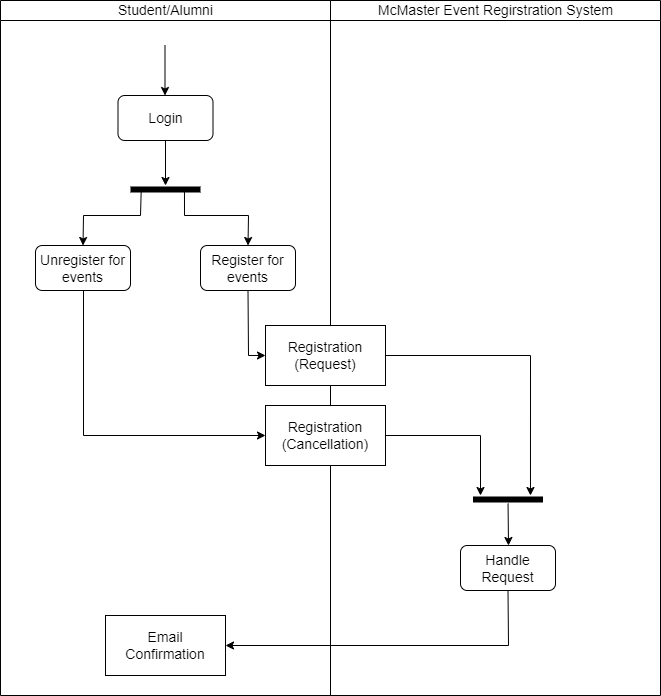
\includegraphics[scale=0.5]{Current_Situation.png}
\end{center}
\caption{Context Diagram}
\end{figure}

\subsection{The Context of the Work}

The context diagram depicted below illustrates the interactions of the system with adjacent external systems and services.
\begin{figure}[H]
\begin{center}
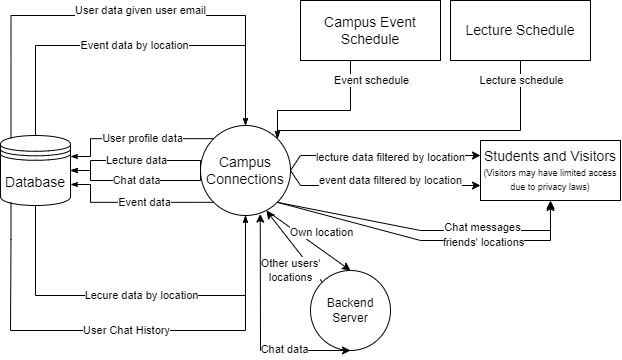
\includegraphics[scale=0.7]{Context_Diagram.png}
\end{center}
\caption{Current Situation}
\end{figure}

\subsection{Work Partitioning}

\begin{table}[H]
  \begin{tabular}{p{0.33\textwidth} | p{0.33\textwidth} | p{0.33\textwidth}}
  \toprule
  \textbf{Event Name} & \textbf{Input/Output} & \textbf{Summary}\\
  \midrule
  Provide lectures list & IN: Lecture schedules & Give a list of lectures when there is an update and after every semester\\
  \midrule
  Provide events list & IN: Event schedules & Give a list of campus events periodically and when there is an update\\
  \midrule
  Record user data & OUT: User data & Record user related data, including user profile, user friends and interested lectures and events\\
  \midrule
  Record lecture data & OUT: Event data & Record lecture data, including lecture name,  time, duration and location\\
  \midrule
    Record event data & OUT: Event data & Record event data, including event name,  time,  duration and location\\
  \midrule
  Display events & IN: event data, OUT: event data filtered by location & Display events that are going to be held in in a given building\\
  \midrule
  Display lectures & IN: lecture data, OUT: lecture data filtered by location & Display lectures that are going to be held in in a given building\\
    \bottomrule
\end{tabular}
 \caption{Business Event List} 
 \label{TblEventList}
\end{table}
\begin{table}[H]
  \begin{tabular}{p{0.33\textwidth} | p{0.33\textwidth} | p{0.33\textwidth}}
  \toprule
    \textbf{Event Name} & \textbf{Input/Output} & \textbf{Summary}\\
  \midrule
  Display user profile & OUT: User profile & Display user profile including user program and level, interested lectures and events\\
    \midrule
  Display map view & OUT: Users' locations & Display the locations of the user and all friends on campus map\\
    \midrule
  Display map view & OUT: Users' locations & Display the locations of the user and all friends on campus map\\
    \midrule
  Display AR view & IN: Target building scene, OUT: AR objects & Display the information and activities of the target building in an AR way\\
  \bottomrule
\end{tabular}
 \caption{Business Event List Cont} 
 \label{TblEventListCont}
\end{table}

\subsection{Specifying a Business Use Case (BUC)}

The following is an activity diagram for the Display event schedule process. The trigger of this business user case will be user interaction, and input will be campus event data from database. What will be displayed is a schedule of events held inside a specific building with detailed event information.
\begin{figure}[H]
\begin{center}
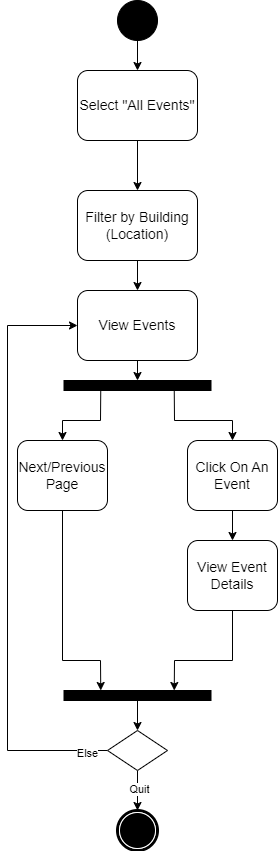
\includegraphics[scale=0.5]{BUC_Activity_Diagram.png}
\end{center}
\caption{Activity diagram for Display Events List Process}
\end{figure}

\section{Business Data Model and Data Dictionary}
\subsection{Business Data Model}

The following UML class diagram shows all types of business data that will be used in this project.\\
All the classes represent corresponding business data, all these entries and their attributes will be defined and explained in the data dictionary.
class are defined in the data dictionary.
\begin{figure}[H]
\begin{center}
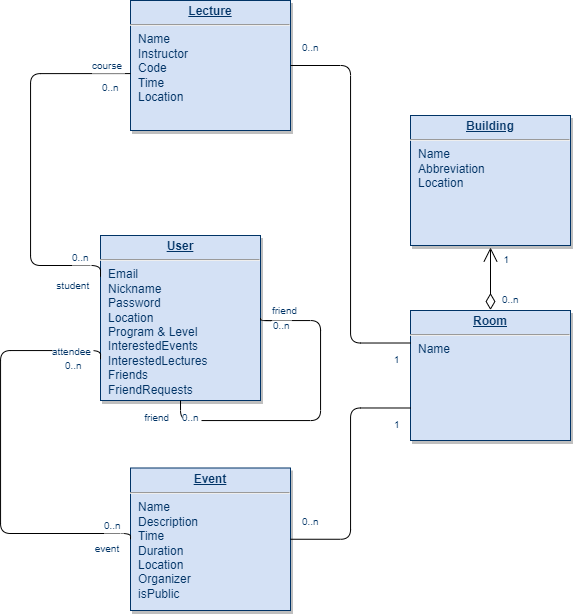
\includegraphics[scale=0.5]{Business_Data_Model.png}
\end{center}
\caption{UML class model}
\end{figure}

\subsection{Data Dictionary}
This section will include definition of all classes in UML class model and their attributes. Some self-explanatory attributes like name will be ignored.
\begin{longtable}
 {p{0.3\textwidth} | p{0.4\textwidth} | p{0.3\textwidth}}
  \toprule
  \textbf{Name} & \textbf{Content} & \textbf{Type}\\
  \midrule
  Lecture & McMaster course data & Class\\
  \midrule
  Lecture.Instructor & Course instructor & Attribute\\
  \midrule
  Lecture.Time & Course schedule & Attribute\\
  \midrule
  Lecture.Location & Course location & Room\\
  \midrule
  Event & McMaster on-campus event data & Class\\
  \midrule
    Event.Description & More information of this event & Attribute\\
  \midrule
  Event.Time & Event time & *HH/MM/SS
24 hour clock*\\
  \midrule
  Event.Location & Event location & Room\\
  \midrule
  Event.Organizer & Held by which department & Attribute\\
  \midrule
  Event.isPublic & Is this event open for non students? & True or False\\
  \midrule
  User & User account data, friends data, location,  event \& lecture attendance & Class\\
  \midrule
  User.Email & email of the user & Attribute\\
  \midrule
  User.Nickname & name displayed in the application & Attribute\\
  \midrule
  User.Password & password of the account & Attribute\\
  \midrule
  User.Location & Geographic location & Attribute\\
  \midrule
  User.InterestedEvents & List of event & Event, Attribute\\
  \midrule
  User.InterestedLectures & List of lecture & Lecture, Attribute\\
  \midrule
  User.Friends & List of friends & User , Attribute\\
  \midrule
  \textbf{Name} & \textbf{Content} & \textbf{Type}\\
  \midrule
  User.FriendRequests & List of users who want to be your friends & User , Attribute\\
  \midrule
  Building & McMaster main campus building & Class\\
  \midrule
  Building.Abbreviation & Abbreviation of building name & Attribute\\
  \midrule
  Building.Location & Geographic location & Attribute\\
  \midrule
  Room & Room inside a building & Class\\
  \midrule
  Room.Name & Room number & Attribute\\
  \bottomrule
  \caption{Data Dictionary} \label{TblDataDict}\\
\end{longtable}

\section{The Scope of the Product}
\subsection{Product Boundary}

The use case diagram depicted below identifies the boundaries between the users and the product.
\begin{figure}[H]
\begin{center}
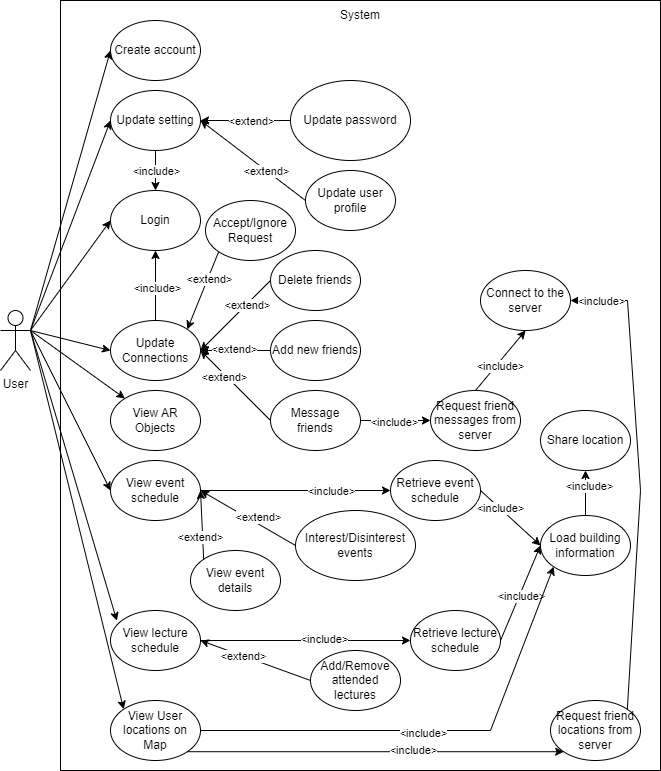
\includegraphics[scale=0.5]{Use_Case_Diagram.png}
\end{center}
\caption{Use Case Diagram}
\end{figure}

\subsection{Product Use Case Table}

\begin{longtable}
 {p{0.1\textwidth} | p{0.4\textwidth} | p{0.2\textwidth} | p{0.3\textwidth}}
  \toprule
  \textbf{PUC No} & \textbf{PUC Name} & \textbf{Actor/s} & \textbf{Input \& Output}\\
  \midrule
  1 & Create Account & User & Email \& Password (in)\\
  \midrule
  \textbf{PUC No} & \textbf{PUC Name} & \textbf{Actor/s} & \textbf{Input \& Output}\\
  \midrule
  2 & Update Password & User & Email \& New Password (in)\\
  \midrule
  3 & Update User Profile & User & New Profile (in)\\
  \midrule
  4 & Login & User & Email \& Password (in),  Response Message (out)\\
   \midrule
  5 & Accept/Ignore Request & User & Friend Email (in), Accept or Ignore message (out)\\
  \midrule
  6 & Add New Friend & User & Friend Email (in), Friend Request (out)\\
  \midrule
  7 & Delete Friend & User & Friend Email (in), Confirmation Message (out)\\
  \midrule
  8 & Message Friend & User & Message Content (in), Message Sent Notification (out)\\
  \midrule
   9 & View AR Objects & User & User Interaction \& target building (in), AR Objects (out)\\
  \midrule
  10 & View Event Details & User & User Interaction (in), Event Details (out)\\
  \midrule
  11 & View Lecture Details & User & User Interaction (in), Lecture Details (out)\\
  \midrule
  12 & Interest/Disinterest Event & User & User Interaction \& Event Name (in)\\
  \midrule
  13 & Add/Remove Lecture & User & User Interaction \& Lecture Name (in)\\
  \midrule
  14 & View User locations on Map & User & User Interaction \& User Locations (out)\\
  \midrule
  \textbf{PUC No} & \textbf{PUC Name} & \textbf{Actor/s} & \textbf{Input \& Output}\\
  \midrule
  15 & Retrieve Event Schedule & System & New Schedule (out)\\
  \midrule
  16 & Retrieve Lecture Schedule & System & New Schedule (out)\\
  \midrule
  17 & Load Building Information & System & Location \& Sensor Data (in),  Building Name (out)\\
  \midrule
  18 & Request friend messages from server & System & Target Email (in),  Messages (out)\\
  \midrule
  19 & Request friend locations from server & System & Target Email (in),  Locations (out)\\
  \midrule
  20 & Connect to server & System & Email (in),  Confirm Message (out)\\
  \bottomrule
  \caption{Product Use Case} \label{TblPUC}\\
\end{longtable}

\subsection{Individual Product Use Cases (PUC's)}
\textbf{Use case \#1:} Create Account\\
\textbf{Precondition:} None\\
\textbf{Trigger:} The user clicks on create account button\\
\textbf{Outcome}
\begin{enumerate}
    \item User provides the required information (email, nickname and password) and agrees with the privacy policy of this application
    \item System verifies all required information has been provided
    \item System securely registers the given information as user information
    \item User is redirected back to the Home page
\end{enumerate}
\textbf{Postcondition:} The user has successfully created an account and account information is stored and secured in a database.


\noindent\\
\textbf{Use case \#2:} Update Password\\
\textbf{Precondition:} The user has already created an account\\
\textbf{Trigger:} The user clicks on change password button\\
\textbf{Outcome}
\begin{enumerate}
	\item User navigates to change password page
    \item User provides old password
    \item User provides new password
    \item System verifies old password is correct and new password is valid
    \item System updates password of current user in the database
    \item User is redirected back to the Home page
\end{enumerate}
\textbf{Postcondition:} The user has successfully changed the password.


\noindent\\
\textbf{Use case \#3:} Update User Profile\\
\textbf{Precondition:} The user has already created an account\\
\textbf{Trigger:} The user clicks on edit profile button\\
\textbf{Outcome}
\begin{enumerate}
	\item User navigates to edit profile page
    \item User updates the profile (nickname, avatar, program, level) to a new one and saves the changes
    \item System updates user profile with updates made by the user and redirects back to the Home page
\end{enumerate}
\textbf{Postcondition:} The user profile has been changed successfully.


\noindent\\
\textbf{Use case \#4:} Login\\
\textbf{Precondition:} The user has already created an account\\
\textbf{Trigger:} The user clicks on login button on the home page\\
\textbf{Outcome}
\begin{enumerate}
	\item User navigates to login page and enters email and password
    \item System verifies all required information has been provided and matches the database record
    \item User is redirected to the home page as a logged-in user
\end{enumerate}
\textbf{Postcondition:} The user has successfully logged in to the created account with all settings and connections loaded from the database.


\noindent\\
\textbf{Use case \#5:} Accept/Ignore Request\\
\textbf{Precondition:} The user has already logged in\\
\textbf{Trigger:} The user directs to request management page\\
\textbf{Outcome}
\begin{enumerate}
    \item User checked the requester email
    \item Destined user accepts/rejects the request
    \item User receives a notification
\end{enumerate}
\textbf{Postcondition:} The user gets a new connection in their friends list.\\
\textbf{Postcondition 2:} The user is rejected and gets a notification about that.


\noindent\\
\textbf{Use case \#6:} Add New Friend\\
\textbf{Precondition:} The user has already logged in\\
\textbf{Trigger:} The user searches for another user and sends a friend request\\
\textbf{Outcome}
\begin{enumerate}
	\item User searches for another user
    \item User sends a friend request
    \item System sends the request with requester email to the destined user
    \item User receives a notification
\end{enumerate}
\textbf{Postcondition:} A new request is added to the target user's request list.\\


\noindent\\
\textbf{Use case \#7:} Delete Friend\\
\textbf{Precondition:} The user has already logged in and has at lease one friend\\
\textbf{Trigger:} The user clicks delete button on friend page\\
\textbf{Outcome}
\begin{enumerate}
	\item User searches for a friend
    \item User deletes the friend
    \item System sends a confirmation prompt
    \item User continues to delete
    \item User receives a notification
\end{enumerate}
\textbf{Postcondition:} The friend is deleted from user's friends list.\\


\noindent\\
\textbf{Use case \#8:} Message Friend\\
\textbf{Precondition:} The user has already logged in and has at lease one friend\\
\textbf{Trigger:} The user texts a friend on friend page\\
\textbf{Outcome}
\begin{enumerate}
	\item User clicks on a friend in the list
    \item User start to text the friend
    \item System sends message to the destined friend
\end{enumerate}
\textbf{Postcondition:} The friend receives a message from the user.\\


\noindent\\
\textbf{Use case \#9:} View AR Object\\
\textbf{Precondition:} The user has already logged in and gets into a target building\\
\textbf{Trigger:} The user turns on the AR camera\\
\textbf{Outcome}
\begin{enumerate}
	\item User directs to AR Camera page and turns on the camera
    \item User scans the surroundings with AR Camera
\end{enumerate}
\textbf{Postcondition:} The user sees corresponding AR objects in target areas.\\


\noindent\\
\textbf{Use case \#10:} View Event Details\\
\textbf{Precondition:} The user has already logged in and there exists some events in the system\\
\textbf{Trigger:} The user clicks on an event from the list\\
\textbf{Outcome}
\begin{enumerate}
	\item User directs to Event List Page
    \item User finds a list of events
    \item User clicks on one of the event
    \item System displays more information about the event
\end{enumerate}
\textbf{Postcondition:} The name, description,  organizer, duration, time and location of the event are displayed.\\


\noindent\\
\textbf{Use case \#11:} View Lecture Details\\
\textbf{Precondition:} The user has already logged in and there exists some letures in the system\\
\textbf{Trigger:} The user clicks on a lecture from the list\\
\textbf{Outcome}
\begin{enumerate}
	\item User directs to Lecture List Page
    \item User finds a list of lectures
    \item User clicks on one of the lecture
    \item System displays more information about the lecture
\end{enumerate}
\textbf{Postcondition:} The name, code,  instructor, time and location of the lecture are displayed.\\


\noindent\\
\textbf{Use case \#12:} Interest/Disinterest Event\\
\textbf{Precondition:} The user has already logged in and clicks on an event in the list\\
\textbf{Trigger:} The user clicks on bookmark/unbookmark button\\
\textbf{Outcome}
\begin{enumerate}
	\item User browses the event list
	\item User navigates to an event detail page with a specific name
	\item User clicks on the corresponding button
    \item System sends the request to the database
    \item System displays the new state of the event
\end{enumerate}
\textbf{Postcondition:} The event is added to/delete from the user correspondingly in the database and the UI changes as well.\\


\noindent\\
\textbf{Use case \#13:} Add/Remove lecture\\
\textbf{Precondition:} The user has already logged in and clicks on a lecture in the list\\
\textbf{Trigger:} The user clicks on bookmark/unbookmark button\\
\textbf{Outcome}
\begin{enumerate}
	\item User browses the lecture list of the target
	\item User navigates to a lecture detail page with a specific course code
	\item User clicks on the corresponding button
    \item System sends the request to the database
    \item System displays the new state of the lecture
\end{enumerate}
\textbf{Postcondition:} The lecture is added to/removed from the user correspondingly in the database is updated and the UI changes correspondingly.\\


\noindent\\
\textbf{Use case \#14:} View User Locations on Map\\
\textbf{Precondition:} The user has already logged and has at least a friend\\
\textbf{Trigger:} The user directs to campus map page\\
\textbf{Outcome}
\begin{enumerate}
	\item User navigates to campus map page
    \item System displays real time locations of the user and friends who are willing to share locations
\end{enumerate}
\textbf{Postcondition:} The user sees real time locations of friends on campus


\noindent\\
\textbf{Use case \#15:} Retrieve Event Schedule\\
\textbf{Precondition:} None\\
\textbf{Trigger:} A request to update schedule is sent or trigger by the system timer\\\
\textbf{Outcome}
\begin{enumerate}
	\item System sends a request to the on-campus schedule interface
    \item System gets the up-to-date schedule
    \item System stores the new schedule to the database or the administrator adds the new schedule to the database
\end{enumerate}
\textbf{Postcondition:} The new schedule is stored in the database and will be utilized later.\\


\noindent\\
\textbf{Use case \#16:} Retrieve Lecture Schedule\\
\textbf{Precondition:} None\\
\textbf{Trigger:} A request to update schedule is sent or trigger by the system timer\\\
\textbf{Outcome}
\begin{enumerate}
	\item System sends a request to lecture schedule interface
    \item System gets the up-to-date schedule
    \item System stores the new schedule to the database or the administrator adds the new schedule to the database
\end{enumerate}
\textbf{Postcondition:} The new schedule is stored in the database and will be utilized later.\\


\noindent\\
\textbf{Use case \#17:} Load Building Information\\
\textbf{Precondition:} Location share is allowed and sensors are set properly\\
\textbf{Trigger:} A request for event/lecture schedule is sent by the user\\
\textbf{Outcome}
\begin{enumerate}
	\item System gets geographic location and sensor data from the device
    \item System finds the most likely building on campus
    \item System displays building information
\end{enumerate}
\textbf{Postcondition:} The system provides information of the building the user locates now.\\


\noindent\\
\textbf{Use case \#18:} Request friend messages from server\\
\textbf{Precondition:} User is connected to the server and has a friend\\
\textbf{Trigger:} The user opens a chat with friend\\
\textbf{Outcome}
\begin{enumerate}
	\item System sends a request to the server to establish a session for message transfer between the user and the friend
    \item System sends a message from the user to the friend
    \item System request a message from the friend to the user
\end{enumerate}
\textbf{Postcondition:} The user can send and receive to any friends.\\


\noindent\\
\textbf{Use case \#19:} Request friend locations from server\\
\textbf{Precondition:} User is connected to the server and has a friend\\
\textbf{Trigger:} The user directs to campus map page\\
\textbf{Outcome}
\begin{enumerate}
	\item System sends a request to the server to establish a session for sending and receiving real time locations
    \item System sends current location of the user
    \item System request current locations of friends
\end{enumerate}
\textbf{Postcondition:} The user can see everyone's real time locations on the map.\\


\noindent\\
\textbf{Use case \#20:} Connect to server\\
\textbf{Precondition:} User is logged in\\
\textbf{Trigger:} The user wants to send or receive any real time data\\
\textbf{Outcome}
\begin{enumerate}
	\item System sends the user email as ID to the server
    \item Server responds with a confirmation message
\end{enumerate}
\textbf{Postcondition:} The user is connected to the server.\\
\textbf{Postcondition 2:} The user fails to connect due to some issues on the server side.\\
\section{Functional Requirements}
\subsection{Pre-Registration Settings}
    \textbf{FR-1-1:} The system shall ask all users to sign a consent form disclosure of personal information when creating a new account.\\
    \textbf{Rationale:} It is a must to ask for users' permission before making use of their personal information.\\
    \textbf{Fit Criterion:} Users must be able to accept or reject a consent form when they register an account.\\\\
    
\subsection{User Profile}
    \textbf{FR-2-1:} The system shall allow users to create accounts with an email that does not exist in the database.\\
    \textbf{Rationale:} Users must be associated with accounts to identify themselves and expand their social networking.\\
    \textbf{Fit Criterion:} Users must be able to create an account with an email that does not exist in the database and a password.\\\\
    \textbf{FR-2-2:} The system shall allow users to delete their accounts with all associated data.\\
    \textbf{Rationale:} Users shall be able to quit whenever they want with all their data handled properly.\\
    \textbf{Fit Criterion:} Users must be able to delete their account once they log into the application.\\\\
    \textbf{FR-2-3:} The system shall allow users to log in with their email and the corresponding password.\\
    \textbf{Rationale:} Users must be able to log into their account to expand social networking and enjoy all functionalities.\\
    \textbf{Fit Criterion:} Users must be able to log in once they created an account successfully.\\\\
    \textbf{FR-2-4:} The system shall allow users to change their password.\\
    \textbf{Rationale:} This will allow users to improve the security of their account and recover the account if they forget their password.\\
    \textbf{Fit Criterion:} Users may request a password reset on the login page. The user shall receive an email to reset the password later.\\\\
     \textbf{FR-2-5:} The system shall allow users to create and change a virtual avatar.\\
    \textbf{Rationale:} A customizable avatar gives users a much stronger feeling of personalization. \\
    \textbf{Fit Criterion:} Users shall be able to upload images as their avatar on the user profile page.\\\\
    \textbf{FR-2-6:} The system shall allow users to verify their school email.\\
    \textbf{Rationale:} Users shall be identified as McMaster students to have full access to all the resources. Therefore identifying McMaster email is necessary. \\
    \textbf{Fit Criterion:} The user shall be able to add McMaster email to their profile and verify the email after receiving an email from the system.\\\\
    \textbf{FR-2-7:} Users shall be able to edit their profile.\\
    \textbf{Rationale:} Users shall always be able to update their displayed information for better socializing.\\
    \textbf{Fit Criterion:} Users shall be able to edit their user profile (e.g. nickname program and level) on the user profile page.\\\\

\subsection{Friend System}
    \textbf{FR-3-1:} The system shall allow users to send a friend request.\\
    \textbf{Rationale:} One of the main purposes of this application is to make students connect with peers easily. For this to happen, they should be able to make new friends on this social media platform.\\
    \textbf{Fit Criterion:} Users can search for other users through username and send a friend request, added friends can be removed from the friend list.\\\\
    \textbf{FR-3-2:} The system shall allow users to delete friends.\\
    \textbf{Rationale:} When users add users as friends by accident or they no longer connect, they should be able to remove them from the friend list.\\
    \textbf{Fit Criterion:} Users can remove any friends from their friend list.\\\\
    \textbf{FR-3-3:} The system shall allow users to send text messages to their friends.\\
    \textbf{Rationale:} This will make the app more interactive and encourage and enhance socialization between users.\\
    \textbf{Fit Criterion:} Users must be able to send messages and view received messages.\\\\
    \textbf{FR-3-4:} The system shall allow users to share events when chatting with friends.\\
    \textbf{Rationale:} This encourages onsite socialization and allows users to make better use of resources provided by the application.\\
    \textbf{Fit Criterion:} Users shall be able to share a link that can redirects to an event from the chat.\\\\
    \textbf{FR-3-5:} The system shall allow users to share lectures when chatting with friends.\\
    \textbf{Rationale:} his encourages onsite socialization and allows users to make better use of resources provided by the application.\\
    \textbf{Fit Criterion:} Users should be able to share a link that can redirects to a lecture from the chat.\\\\
    \textbf{FR-3-6:} The system shall allow users to manage friend requests.\\
    \textbf{Rationale:} Managing friend requests is a significant functionality to make new friends.\\
    \textbf{Fit Criterion:} Users can either accept or ignore any friend requests.\\\\

\subsection{Lectures and Events}
    \textbf{FR-4-1:} The system shall allow users to manage events they are interested in.\\
    \textbf{Rationale:} It will be much easier for users to find events they are interested in and willing to join again. So that they do not have to browse the event list again and again. While their friends can see what events they are likely to join.\\
    \textbf{Fit Criterion:} Users should be able to save and unsave an event from the event list, this event will be displayed or removed on the user profile page.\\\\
    \textbf{FR-4-2:} The system shall allow users to manage lectures they are interested in.\\
    \textbf{Rationale:} Sharing schedules with friends can strengthen friendship. Users can join lectures with friends and know their classmates better. So the system needs to have the functionality to save lectures.\\
    \textbf{Fit Criterion:} Users should be able to save and unsave a lecture from the list, this lecture will be displayed or removed on the user profile page.\\\\
    \textbf{FR-4-3:} The system shall allow users with an administrator account to add, edit, and remove events.\\
    \textbf{Rationale:} The event information must be up-to-date and accurate. The administrator account will maintain all events so that there is a singular source of information. Additionally, this reduces the chances of errors being introduced to the system.\\
    \textbf{Fit Criterion:} A new event can be created only by a user who is logged in as an administrator. The information for those events can be changed only by administrators. Events can be deleted only by administrators.\\\\
    \textbf{FR-4-4:} The system shall allow users with an administrator account to add, edit, and remove lectures from the schedule.\\
    \textbf{Rationale:} The lecture information must be up-to-date and accurate as well. Administrators are needed to manage the schedule.\\
    \textbf{Fit Criterion:} A lecture on the schedule can be created, deleted, or updated by a user who logged in as an administrator.\\\\
    \textbf{FR-4-5:} Each event shall be associated with an organizer (club/department), location, time and duration.\\
    \textbf{Rationale:} For the application to schedule events for the users to see and interact with, all specific details about the event should be provided to the system\\
    \textbf{Fit Criterion:} When a department/club requests for an event to be posted on the application, they have to provide details about the building and room number it will be held in, along with the date and time the event will take place at.\\\\
    \textbf{FR-4-6:} Each lecture shall be associated with an instructor, location, course code and time.\\
    \textbf{Rationale:} To find empty rooms and help users who want to attend specific lectures, all details about the lectures should be provided to the system.\\
    \textbf{Fit Criterion:} When a lecture is added or modified, all the details mentioned above must be set as mandatory fields.\\\\
    \textbf{FR-4-7:} User should be able to filter specific lectures out from the list by course code.\\
    \textbf{Rationale:} It is necessary to allow users to filter out lectures they are interested in from a long list.\\
    \textbf{Fit Criterion:} Users shall be able to input some keywords to filter the lecture list.\\\\
    \textbf{FR-4-8:} User should be able to filter specific events out from the list by name.\\
    \textbf{Rationale:} It is necessary to allow users to filter out events they are interested in from a long list.\\
    \textbf{Fit Criterion:} Users shall be able to input some keywords to filter the event list.\\\\

\subsection{AR Camera}
    \textbf{FR-5-1:} The system shall recognize specific buildings on campus.\\
    \textbf{Rationale:} AR camera will give users an immersive user experience interacting with campus buildings.\\
    \textbf{Fit Criterion:} The system shall recognize proper camera input as buildings in the database.\\\\
    \textbf{FR-5-2:} The system shall display corresponding event/lecture information as AR objects when a target is recognized.\\
    \textbf{Rationale:} AR camera will give users an immersive user experience interacting with campus buildings.\\
    \textbf{Fit Criterion:} User must see corresponding information about the target (e.g. events and lectures) in the format of AR objects once a target is recognized.\\\\

\subsection{Map and Location}
    \textbf{FR-6-1:} The system shall allow users to see their own real-time locations on campus and the locations of friends who are willing to share.\\
    \textbf{Rationale:} Sharing locations with connections can make it easier for friends to sync up in person on campus, which provides more opportunities for users to network\\
    \textbf{Fit Criterion:} Users shall be able to see a yellow pin on the map showing their real-time positions, and also other users' and locations represented by blue pins, on campus.\\\\

\section{Look and Feel Requirements}
\subsection{Appearance Requirements}
  \textbf{LF-A1:} The product shall respond with visual (and auditory, if applicable) feedback once the user interacts with an interactive component.\\
  \textbf{Rationale:} Providing feedback will tell the user that the product has done a task in response to the user input.\\
  \textbf{Fit criterion:} Each interactive component responds to user input within RESPONSE\_TIME seconds, either by opening a dialog or altering the visual state. If sound feedback is incorporated, it plays within the same time frame.\\\\
  \textbf{LF-A2:} The product shall adapt to most of the common mobile screen sizes with screen components not being congested.\\
  \textbf{Rationale:} This will allow the user to view and interact with all the visual elements on the page.\\
  \textbf{Fit criterion:} Visual elements must not exceed the borders of the screen for all screens in SCREEN\_VIEWPORTS list. If a user experience survey is taken among them, the application layout will get at least MIN\_SCORE.\\

\subsection{Style Requirements}
  \textbf{LF-S1:} The colors and themes shall be consistent across different pages.\\
  \textbf{Rationale:} Colours should be consistent to allow the user to easily navigate each page.\\
  \textbf{Fit criterion:} Consistency checks show the same color scheme being used on all pages.\\\\
  \textbf{LF-S2:} The color scheme used shall be appealing and not cause eye strain.\\
  \textbf{Rationale:} An unappealing colour scheme may cause eye strain in users.\\
  \textbf{Fit criterion:} MOST\_USERS agree with the statement that the screen does not cause strain during a user experience survey. MOST\_USERS also agree that the color scheme is visually appealing.\\

\section{Usability and Humanity Requirements}
\subsection{Ease of Use Requirements}
  \textbf{UH-EOU1:} The product shall have a user interface that is clear and easy to navigate.\\
  \textbf{Rationale:} A user interface that is easy to use will allow users to intuitively navigate between pages without any assistance.\\
  \textbf{Fit criterion:} MOST\_USERS in the usability testing stage shall be able to find their way to specific pages and access all different core features including messaging friend, lecture and event management and building scanning without needing to try again more than 3 times.\\

\subsection{Personalization and Internationalization Requirements}
  \textbf{N/A}\\

\subsection{Learning Requirements}
  \textbf{UH-L1:} The product shall include a user guide about its features available on GitHub repo.\\
  \textbf{Rationale:} This will aid users in navigating the user interface if a user is unable to find a feature.\\
  \textbf{Fit criterion:} Users shall be able to access user guide in GitHub and MOST\_USERS shall give positive feedback on that document.\\\\

\subsection{Understandability and Politeness Requirements}
  \textbf{UH-UP1:} The product shall abstain from using technical and software-specific language.\\
  \textbf{Rationale:} Technical and software-specific language will not be understood by most users, therefore its use should be limited.\\
  \textbf{Fit criterion:} MOST\_USERS shall not find technical and software-specific language among all text displayed by the application.\\
\subsection{Accessibility Requirements}
  \textbf{UH-A1:} The colors used by the different components of the product shall contrast enough for items on the screen to be more easily visible.\\
  \textbf{Rationale:} This will allow users with colour blindness to tell different components apart, as colours with low contrast may be hard to distinguish for these users.\\
  \textbf{Fit criterion:} The color contrast is at least 4.5:1 per the Web Content Accessibility Guidelines’ AA standards for accessibility\cite{WCAG}.\\

\section{Performance Requirements}
\subsection{Speed and Latency Requirements}
  \textbf{P-SL1:} The product shall display the correct AR objects shortly after successful AR target recognition.\\
  \textbf{Rationale:} Response times should be fast to ensure that the product is efficient.\\
  \textbf{Fit criterion:} The time from recognition to the appearance of the AR object is at most RECOGNITION\_TIME.\\\\
  \textbf{P-SL2:} The product shall periodically update the user’s location on the real-time location map.\\
  \textbf{Rationale:} User's location should be as accurate as possible. Constant updates will ensure that the user's location is up to date.\\
  \textbf{Fit criterion:} A user’s location must be updated on the map session within LOCATION\_UPDATE\_TIME.\\

\subsection{Safety-Critical Requirements}
 \textbf{N/A}
\subsection{Precision or Accuracy Requirements}
  \textbf{P-PA1:} The product shall accurately identify building targets scanned by the user.\\
  \textbf{Rationale:} When a user scans a valid building target, the product should display interactive visual elements with information about that building\\
  \textbf{Fit criterion:} The application shall correctly identify an indoor or outdoor building target within 2 seconds 80\% of the time under clear conditions (not obscured by objects or in poor lighting).\\\\

\subsection{Robustness or Fault-Tolerance Requirements}
  \textbf{\textcolor{red}{P-RF1 (No Longer Valid Due To Scope Change):}} The product shall display an error message when there is no internet connection.\\
  \textbf{Rationale:} When there is no internet connection, the user should be made aware. (Note: Due to a change in scope, this requirement is no longer valid)\\
  \textbf{Fit criterion:} An error message stating that there is no internet connection is displayed when the product fails to connect to the internet.\\\\
  \textbf{P-RF2:} There must be a fail-safe for the product to function if the server connection takes too long or fails.\\
  \textbf{Rationale:} This will allow the product to function to some degree even during high traffic or bad server connection situations.\\
  \textbf{Fit Criterion:} The product must be able to provide rudimentary functionalities without connecting to the server.\\\\
  \textbf{P-RF3:} The server shall attempt to restart when it crashes.\\
  \textbf{Rationale:} This requirement enhances the robustness of the backend server and prevents it from going down for a long time because of some intermittent minor errors.\\
  \textbf{Fit Criterion:} The server shall restart the instance if it crashes due to an unrecoverable error.\\\\
  \textbf{P-RF4:} AR Camera should have a notification available in the UI telling users possible reasons the target is not recognized.\\
  \textbf{Rationale:} The user should get a notification telling them that the AR camera may have a bad performance in some cases, and they should be able to report that to the developer if they want the problem to be solved.\\
  \textbf{Fit Criterion:} The product should show the user a list of possible reasons that the camera does not work and the contact information of maintainers once they have trouble using the AR camera and click the help button.\\\\

\subsection{Capacity Requirements}
  \textbf{N/A}\\

\subsection{Scalability or Extensibility Requirements}
  \textbf{P-SE1:} The product shall have a server that can process all users.\\
  \textbf{Rationale:} Ensures that the app can handle the requests of multiple users at once.\\
  \textbf{Fit Criterion:} The server should be capable of processing at most MAX\_CAPACITY people concurrently in the release build with a plan of expanding it to support all students on campus (about 40,000 people) in the future.\\\\
  \textbf{P-SE2:} The product shall have a database that can store the information of all users.\\
  \textbf{Rationale:} Ensures that all user's information can be stored in the database\\
  \textbf{Fit Criterion:} The database should be capable of storing the account and personal information of about MAX\_USER\_STORED users in the release build with a plan of expanding it to support all students on campus (about 40,000 people) in the future.\\\\
  \textbf{P-SE3:} The application architecture shall allow for the addition of new campus buildings and clubs without considerable drawbacks in performance.\\
  \textbf{Rationale:} New buildings and clubs may be added in future releases.\\
  \textbf{Fit Criterion:} New buildings and clubs can be added to the database within a few minutes, and their addition causes minimal increase in processing delay.\\\\

\subsection{Longevity Requirements}
  \textbf{P-L1:} This application shall operate without major malfunctions in release build while undergoing further development.\\
  \textbf{Rationale:} This will ensure that new releases can be focused on without worrying about any malfunctions in the current release.\\
  \textbf{Fit Criterion:} The application will be expected to operate for a minimum of 1 year after release.\\\\
  \textbf{P-L2:} The finalized product shall remain compatible with the promised supported operating systems and devices.\\
  \textbf{Rationale:} Ensures that users can use the app for a sufficient amount of time without having to get a new phone.\\
  \textbf{Fit Criterion:} The product should be compatible with supported devices for a minimum of 3 years.\\\\

\section{Operational and Environmental Requirements}
\subsection{Expected Physical Environment}
  \textbf{OE-EPE1:} The product shall be installed on the user's smartphone (Android).\\
  \textbf{Rationale:} The product is a mobile phone application.\\
  \textbf{Fit Criterion:} The product can be opened from the user's home screen once downloaded.\\\\

\subsection{Wider Environment Requirements}
  \textbf{N/A}\\

\subsection{Requirements for Interfacing with Adjacent Systems}
  \textbf{N/A}\\

\subsection{Productization Requirements}
  \textbf{OE-P1:} The product shall be downloadable for Android devices.\\
  \textbf{Rationale:} The expected physical environment is Android devices.\\
  \textbf{Fit criterion:} The product can be downloaded onto an Android device by downloading the APK file directly.\\\\

\subsection{Release Requirements}
  \textbf{N/A}\\

\section{Maintainability and Support Requirements}
\subsection{Maintenance Requirements}
  \textbf{MS-M1:} Major updates could be rolled out during periods of reduced usage such as after school time in the midnight, in the Reading Week or Spring/Summer semesters.\\
  \textbf{Rationale:} This minimizes the number of users that are impacted by ongoing maintenance.\\
  \textbf{Fit Criterion:} Dates and times of update releases correspond with days/times that are expected to have lower usage.\\\\
  %This will allow significant time to stablize the update and test them before the updates are applied to the users.
  %Additionally, the administrator can perfrom maintenance on the database and server to check the correct operation of the product.
  %This will maximize the availability of the product.

\subsection{Supportability Requirements}
  \textbf{MS-S1:} Feature requests or issues can be sent to the application's GitHub.\\
  \textbf{Rationale:} This will allow users to report bugs/suggest new features to the developers.\\
  \textbf{Fit Criterion:} A link for the application's GitHub will be provided to users, allowing them to add feature requests or issues.\\\\
  %These opened issues will be discussed by the maintainers and communicated through the issue on how they will be dealt with.
  \textbf{MS-S2:} The user manual and all feature issues with implementation details should be open to any visitor to the application's GitHub.\\
  \textbf{Rationale:} Users should have access to the user manual to aid them in using the application. Feature issues should also be made public so users can see the progress being made.\\
  \textbf{Fit Criterion:} The user manual and feature issues shall be viewable by any user with/without a GitHub account.\\\\

\subsection{Adaptability Requirements}
  \textbf{MS-A1:} The product shall be accessible on Android 11 and above for Android devices.\\
  \textbf{Rationale:} These operating systems are still supported and receive security updates.\\
  \textbf{Fit Criterion:} In a sample of 10 phones running Android 11 or later, at least 9 should be capable of running the application without encountering unexpected issues.\\\\
  %This product may be ported to other universities in Ontario, Canada, or other countries.
  %Although the product is designed to work for university, this can be porte to other large events and buildings to help users navigate and coordinate better.

\section{Security Requirements}
\subsection{Access Requirements}
  \textbf{S-A1:} User with first level access is treated as a guest.\\
  \textbf{Rationale:} User persona: a grade 12 student on a university tour.\\
  \textbf{Fit Criterion:} Guest must not have access to anything beyond the login, account creation, public events, user profile and campus map (without other users' locations) pages. \\\\
  \textbf{S-A2:} User with second level access is treated as an actual user (student).\\
  \textbf{Rationale:} User persona: a software engineer undergrad student.\\
  \textbf{Fit Criterion:} User will have full access to all features except writing access to the database, which means a user cannot edit or create new lectures or events. \\\\
  \textbf{S-A3:} User with thrid level access is treated as an administrator.\\
  \textbf{Rationale:} User persona: a staff of engineering faculty. Full access of the system should be given to administrators who works as a maintainer.\\
  \textbf{Fit Criterion:} Administrator will have all the access users have and the power to add, delete and edit official events, lectures and all users profiles.\\\\
    \textbf{S-A4:} The product shall prevent the user from entering special characters in all text input fields.\\
  \textbf{Rationale:} When creating accounts, users can perform SQL injection attacks by inputting some SQL statements.\\
  \textbf{Fit Criterion:} Any text input with special characters will give the user an error.\\\\
  \textbf{S-A5:} The product shall validate the email format when creating an account.\\
  \textbf{Rationale:} The format of the input should be validated to ensure no errors occur and no malicious attacks can be executed.\\
  \textbf{Fit Criterion:} All emails in the database should have a email format, an input in the email field that's not in the format of an email will give the user an error when creating a new account.\\
  $(\forall\; email \in DB\;  |\;  email.Match([A-Z0-9+\_.-]+@[A-Z0-9.-]+)$\\\\

\subsection{Integrity Requirements}
  \textbf{N/A}\\

\subsection{Privacy Requirements}
  \textbf{S-P1:} The application will comply with all relevant privacy laws and guidelines.\\
  \textbf{Rationale:} The application will respect the privacy of all the users.\\
  \textbf{Fit Criterion:} The usage of a user's personal information by the product abides by the Privacy Act, The Personal Information Protection and Electronic Documents Act, and Canada and Ontario’s data protection laws \cite{Legislative Services} \cite{CFLC}. More specificly, since the application does not match any of the exceptions in Division 1 Protection of Personal Information in Personal Information Protection and Electronic Documents Act, the application must not do the following: 7.1) Collection without knowledge or consent; 7.2) Use without knowledge or consent; 7.3) Disclosure without knowledge or consent\\\\
  \textbf{S-P2:} Accounts that are inactive for a certain period shall be deleted to prevent unnecessary data from being held.\\
  \textbf{Rationale:} It prevents personal information from being stored in the database unintentionally for a long time.\\
  \textbf{Fit Criterion:} Accounts that are not logged in for a semester will be cleaned from the authentication system and database.\\\\
  \textbf{S-P3:} The application will not collect or share any user’s location or personal data without getting permission from the user.\\
  \textbf{Rationale:} This gives the user the freedom to choose how their personal data is used by the product.\\
  \textbf{Fit criterion:} User’s personal information does not appear in the database if the user did not grant permissions.\\\\
  \textbf{S-P4:} User data such as messages and location information will be securely encrypted to protect user’s privacy.\\
  \textbf{Rationale:} This decreases the risk of hackers finding personal information in intercepted messages.\\
  \textbf{Fit criterion:} An explicit encryption is used so that contents of data packets being transmitted are not readable or decryptable.\\\\
  \textbf{S-P5:} The product shall hide user's location if the user leaves campus.\\
  \textbf{Rationale:} Users may stay connected and share their location even when they leave the campus. To prevent personal information leakage, we need to hide that information and disconnect the user.\\
  \textbf{Fit Criterion:} A user's information shall not be shared once he or she leaves campus.


\subsection{Audit Requirements}
  \textbf{N/A} (This currently does not apply, once the application is ready to be used in multiple universities and regions, audit requirements will be reconsidered.)\\

\subsection{Immunity Requirements}
  \textbf{N/A} (This currently does not apply, once the application is ready to be used in multiple universities and regions, audit requirements will be reconsidered.)\\
  
\subsection{User Safety Requirements}
 \textbf{S-US1:} The product shall display a message upon map startup warning the user to be aware of their surroundings.\\
  \textbf{Rationale:} The real-time location map may be distracting to users, therefore we need to warn the user for their safety.\\
  \textbf{Fit Criterion:} A message telling the user to be aware of their surroundings is displayed upon map startup.\\\\

\section{Cultural Requirements}
\subsection{Cultural Requirements}
  \textbf{CUL-C1:} The product shall not be offensive to any marginalized groups.\\
  \textbf{Rationale:} The app is meant to be used by students on campus, many of which are part of marginalized groups.\\
  \textbf{Fit Criterion:} MOST\_USERS that self-identify as a minority agree that the app does not use any offensive language or symbols.\\\\

\section{Compliance Requirements}
\subsection{Legal Requirements}
  \textbf{COM-L1:} The data collected from users shall be handled as per the same legal requirements set by the university.\\
  \textbf{Rationale:} The university has specific privacy policy on Collection of Personal Information and Protection of Privacy\cite{Privacy} that must be followed.\\
  \textbf{Fit Criterion:} The application does not violate the Disclosure of personal information set by the university in the statement when collecting user data and will only collect data to serve student better as state in General uses of personal information h) in the statement.\\\\
  %As this application will be used in university, it is subject to the same regulations that the university is beholden to.
  %In the future, different functions can be developed to match specific university or state/country requirements, but this is currently not in scope.

\subsection{Standards Compliance Requirements}
  %This ensures that the application is safe and can be scaled and expanded to other universities or interested parties when needed.
  \textbf{COM-SC1:} The application shall abide by the guidelines set by the university and club managers, adding options to accommodate their requests.\\
  \textbf{Rationale:} The university and club managers has specific guidelines for the application that must be followed.\\
  \textbf{Fit Criterion:} The application does not violate any guidelines set by the university and club managers.\\\\

\section{Traceability Matrix}
\begin{table}[H]
  \scalebox{0.7}{
  \begin{tabular}{c|c|c|c|c|c|c|c|c|c|c|c|c|c|c|c|c|c|c|c|c|}
  \cline{2-21}
  \multicolumn{1}{r|}{\textbf{PUC No}}   & \textbf{1}   & \textbf{2}   & \textbf{3}   & \textbf{4}   & \textbf{5}   & \textbf{6}   & \textbf{7}   & \textbf{8}   & \textbf{9}   & \textbf{10}  & \textbf{11}  & \textbf{12}  & \textbf{13}  & \textbf{14}  & \textbf{15}  & \textbf{16}  & \textbf{17}  & \textbf{18}  & \textbf{19}  & \textbf{20}  \\ \hline
  \multicolumn{1}{|l|}{\textbf{FR-1-1}}  &       X      &              &              &              &              &              &              &              &              &              &              &              &              &              &              &              &              &              &              &              \\ \hline
  \multicolumn{1}{|l|}{\textbf{FR-2-1}}  &       X      &              &              &              &              &              &              &              &              &              &              &              &              &              &              &              &              &              &              &              \\ \hline
  \multicolumn{1}{|l|}{\textbf{FR-2-2}}  &       X      &              &              &              &              &              &              &              &              &              &              &              &              &              &              &              &              &              &              &              \\ \hline
  \multicolumn{1}{|l|}{\textbf{FR-2-3}}  &              &              &              &       X      &              &              &              &              &              &              &              &              &              &              &              &              &              &              &              &              \\ \hline
  \multicolumn{1}{|l|}{\textbf{FR-2-4}}  &              &       X      &              &              &              &              &              &              &              &              &              &              &              &              &              &              &              &              &              &              \\ \hline
  \multicolumn{1}{|l|}{\textbf{FR-2-5}}  &              &              &       X      &              &              &              &              &              &              &              &              &              &              &              &              &              &              &              &              &              \\ \hline
  \multicolumn{1}{|l|}{\textbf{FR-2-6}}  &       X      &              &              &              &              &              &              &              &              &              &              &              &              &              &              &              &              &              &              &              \\ \hline
  \multicolumn{1}{|l|}{\textbf{FR-2-7}}  &              &              &       X      &              &              &              &              &              &              &              &              &              &              &              &              &              &              &              &              &              \\ \hline
  \multicolumn{1}{|l|}{\textbf{FR-3-1}}  &              &              &              &              &              &       X      &              &              &              &              &              &              &              &              &              &              &              &              &              &              \\ \hline
  \multicolumn{1}{|l|}{\textbf{FR-3-2}}  &              &              &              &              &              &              &       X      &              &              &              &              &              &              &              &              &              &              &              &              &              \\ \hline
  \multicolumn{1}{|l|}{\textbf{FR-3-3}}  &              &              &              &              &              &              &              &       X      &              &              &              &              &              &              &              &              &              &       X      &              &       X      \\ \hline
  \multicolumn{1}{|l|}{\textbf{FR-3-4}}  &              &              &              &              &              &              &              &       X      &              &              &              &              &              &              &              &              &              &       X      &              &       X      \\ \hline
  \multicolumn{1}{|l|}{\textbf{FR-3-5}}  &              &              &              &              &              &              &              &       X      &              &              &              &              &              &       X      &              &              &              &              &       X      &       X      \\ \hline
  \multicolumn{1}{|l|}{\textbf{FR-3-6}}  &              &              &              &              &       X      &              &              &              &              &              &              &              &              &              &              &              &              &              &              &              \\ \hline
  \multicolumn{1}{|l|}{\textbf{FR-4-1}}  &              &              &              &              &              &              &              &              &              &       X      &              &       X      &              &              &       X      &              &              &              &              &              \\ \hline
  \multicolumn{1}{|l|}{\textbf{FR-4-2}}  &              &              &              &              &              &              &              &              &              &              &       X      &              &       X      &              &              &       X      &              &              &              &              \\ \hline
  \multicolumn{1}{|l|}{\textbf{FR-4-3}}  &              &              &              &              &              &              &              &              &              &       X      &              &              &              &              &       X      &              &              &              &              &              \\ \hline
  \multicolumn{1}{|l|}{\textbf{FR-4-4}}  &              &              &              &              &              &              &              &              &              &              &       X      &              &              &              &              &       X      &              &              &              &              \\ \hline
  \multicolumn{1}{|l|}{\textbf{FR-4-5}}  &              &              &              &              &              &              &              &              &              &       X      &              &              &              &              &       X      &              &              &              &              &              \\ \hline
  \multicolumn{1}{|l|}{\textbf{FR-4-6}}  &              &              &              &              &              &              &              &              &              &              &       X      &              &              &              &              &       X      &              &              &              &              \\ \hline
  \multicolumn{1}{|l|}{\textbf{FR-4-7}}  &              &              &              &              &              &              &              &              &              &       X      &              &              &              &              &       X      &              &              &              &              &              \\ \hline
  \multicolumn{1}{|l|}{\textbf{FR-4-8}}  &              &              &              &              &              &              &              &              &              &              &       X      &              &              &              &              &       X      &              &              &              &              \\ \hline
  \multicolumn{1}{|l|}{\textbf{FR-5-1}}  &              &              &              &              &              &              &              &              &       X      &              &              &              &              &              &              &              &       X      &              &              &              \\ \hline
  \multicolumn{1}{|l|}{\textbf{FR-5-2}}  &              &              &              &              &              &              &              &              &       X      &              &              &              &              &              &              &              &       X      &              &              &              \\ \hline
  \multicolumn{1}{|l|}{\textbf{FR-6-1}}  &              &              &              &              &              &              &              &              &              &              &              &              &              &       X      &              &              &              &              &              &       X      \\ \hline
  \end{tabular}
  }
\caption{Traceability Matrix for PUCs and FRs}
    \label{tab:matrix-puc-fr}
\end{table}

\begin{table}[H]
  \begin{adjustwidth}{-1.4in}{-1in}
  \scalebox{0.7}{
  \begin{tabular}{c|c|c|c|c|c|c|c|c|c|c|c|c|c|c|c|c|c|c|c|c|c|c|c|c|c|}
  \cline{2-26}
  \multicolumn{1}{r|}{\textbf{FR}}       & \textbf{1-1} & \textbf{2-1} & \textbf{2-2} & \textbf{2-3} & \textbf{2-4} & \textbf{2-5} & \textbf{2-6} & \textbf{2-7} & \textbf{3-1} & \textbf{3-2} & \textbf{3-3} & \textbf{3-4} & \textbf{3-5} & \textbf{3-6} & \textbf{4-1} & \textbf{4-2} & \textbf{4-3} & \textbf{4-4} & \textbf{4-5} & \textbf{4-6} & \textbf{4-7} & \textbf{4-8} & \textbf{5-1} & \textbf{5-2} & \textbf{6-1}  \\ \hline
  \multicolumn{1}{|l|}{\textbf{LF-A1}}   &       X      &       X      &       X      &       X      &       X      &       X      &       X      &       X      &       X      &       X      &       X      &       X      &       X      &       X      &       X      &       X      &       X      &       X      &              &              &       X      &       X      &              &       X      &       X       \\ \hline
  \multicolumn{1}{|l|}{\textbf{LF-A2}}   &       X      &       X      &       X      &       X      &       X      &       X      &       X      &       X      &       X      &       X      &       X      &       X      &       X      &       X      &       X      &       X      &       X      &       X      &              &              &       X      &       X      &              &       X      &       X       \\ \hline
  \multicolumn{1}{|l|}{\textbf{LF-S1}}   &       X      &       X      &       X      &       X      &       X      &       X      &       X      &       X      &       X      &       X      &       X      &       X      &       X      &       X      &       X      &       X      &       X      &       X      &              &              &       X      &       X      &              &       X      &       X       \\ \hline
  \multicolumn{1}{|l|}{\textbf{LF-S2}}   &       X      &       X      &       X      &       X      &       X      &       X      &       X      &       X      &       X      &       X      &       X      &       X      &       X      &       X      &       X      &       X      &       X      &       X      &              &              &       X      &       X      &              &       X      &       X       \\ \hline
  \multicolumn{1}{|l|}{\textbf{UH-EOU1}} &       X      &       X      &       X      &       X      &       X      &       X      &       X      &       X      &       X      &       X      &       X      &       X      &       X      &       X      &       X      &       X      &       X      &       X      &              &              &       X      &       X      &              &       X      &       X       \\ \hline
  \multicolumn{1}{|l|}{\textbf{UH-L1}}   &       X      &       X      &       X      &       X      &       X      &       X      &       X      &       X      &       X      &       X      &       X      &       X      &       X      &       X      &       X      &       X      &       X      &       X      &       X      &       X      &       X      &       X      &       X      &       X      &       X       \\ \hline
  \multicolumn{1}{|l|}{\textbf{UH-UP1}}  &       X      &       X      &       X      &       X      &       X      &       X      &       X      &       X      &       X      &       X      &       X      &       X      &       X      &       X      &       X      &       X      &       X      &       X      &              &              &       X      &       X      &              &       X      &       X       \\ \hline
  \multicolumn{1}{|l|}{\textbf{UH-A1}}   &       X      &       X      &       X      &       X      &       X      &       X      &       X      &       X      &       X      &       X      &       X      &       X      &       X      &       X      &       X      &       X      &       X      &       X      &              &              &       X      &       X      &              &       X      &       X       \\ \hline
  \multicolumn{1}{|l|}{\textbf{P-SL1}}   &              &              &              &              &              &              &              &              &              &              &              &              &              &              &              &              &              &              &              &              &              &              &       X      &       X      &               \\ \hline
  \multicolumn{1}{|l|}{\textbf{P-SL2}}   &              &              &              &              &              &              &              &              &              &              &              &              &       X      &              &              &              &              &              &              &              &              &              &              &              &       X       \\ \hline
  \multicolumn{1}{|l|}{\textbf{P-PA1}}   &              &              &              &              &              &              &              &              &              &              &              &              &              &              &              &              &              &              &              &              &              &              &       X      &       X      &               \\ \hline
  \multicolumn{1}{|l|}{\textbf{\textcolor{red}{P-RF1}}}   &              &              &              &              &              &              &              &              &              &              &              &              &              &              &              &              &              &              &              &              &              &              &              &              &               \\ \hline
  \multicolumn{1}{|l|}{\textbf{P-RF2}}   &              &              &              &              &              &              &              &              &              &              &       X      &       X      &       X      &              &              &              &              &              &              &              &              &              &              &              &       X       \\ \hline
  \multicolumn{1}{|l|}{\textbf{P-RF3}}   &              &              &              &              &              &              &              &              &              &              &       X      &       X      &       X      &              &              &              &              &              &              &              &              &              &              &              &       X       \\ \hline
  \multicolumn{1}{|l|}{\textbf{P-RF4}}   &              &              &              &              &              &              &              &              &              &              &              &              &              &              &              &              &              &              &              &              &              &              &       X      &       X      &               \\ \hline
  \multicolumn{1}{|l|}{\textbf{P-SE1}}   &              &              &              &              &              &              &              &              &              &              &       X      &       X      &       X      &              &              &              &              &              &              &              &              &              &              &              &       X       \\ \hline
  \multicolumn{1}{|l|}{\textbf{P-SE2}}   &              &       X      &              &              &              &       X      &              &              &       X      &              &              &              &              &       X      &       X      &       X      &       X      &       X      &              &              &              &              &              &              &               \\ \hline
  \multicolumn{1}{|l|}{\textbf{P-SE3}}   &              &              &              &              &              &              &              &              &              &              &              &              &              &              &              &              &              &              &              &              &              &              &       X      &       X      &               \\ \hline
  \multicolumn{1}{|l|}{\textbf{P-L1}}    &       X      &       X      &       X      &       X      &       X      &       X      &       X      &       X      &       X      &       X      &       X      &       X      &       X      &       X      &       X      &       X      &       X      &       X      &       X      &       X      &       X      &       X      &       X      &       X      &       X       \\ \hline
  \multicolumn{1}{|l|}{\textbf{P-L2}}    &       X      &       X      &       X      &       X      &       X      &       X      &       X      &       X      &       X      &       X      &       X      &       X      &       X      &       X      &       X      &       X      &       X      &       X      &       X      &       X      &       X      &       X      &       X      &       X      &       X       \\ \hline
  \multicolumn{1}{|l|}{\textbf{OE-EPE1}} &       X      &       X      &       X      &       X      &       X      &       X      &       X      &       X      &       X      &       X      &       X      &       X      &       X      &       X      &       X      &       X      &       X      &       X      &       X      &       X      &       X      &       X      &       X      &       X      &       X       \\ \hline
  \multicolumn{1}{|l|}{\textbf{OE-P1}}   &       X      &       X      &       X      &       X      &       X      &       X      &       X      &       X      &       X      &       X      &       X      &       X      &       X      &       X      &       X      &       X      &       X      &       X      &       X      &       X      &       X      &       X      &       X      &       X      &       X       \\ \hline
  \multicolumn{1}{|l|}{\textbf{MS-M1}}   &       X      &       X      &       X      &       X      &       X      &       X      &       X      &       X      &       X      &       X      &       X      &       X      &       X      &       X      &       X      &       X      &       X      &       X      &       X      &       X      &       X      &       X      &       X      &       X      &       X       \\ \hline
  \multicolumn{1}{|l|}{\textbf{MS-S1}}   &       X      &       X      &       X      &       X      &       X      &       X      &       X      &       X      &       X      &       X      &       X      &       X      &       X      &       X      &       X      &       X      &       X      &       X      &       X      &       X      &       X      &       X      &       X      &       X      &       X       \\ \hline
  \multicolumn{1}{|l|}{\textbf{MS-S2}}   &       X      &       X      &       X      &       X      &       X      &       X      &       X      &       X      &       X      &       X      &       X      &       X      &       X      &       X      &       X      &       X      &       X      &       X      &       X      &       X      &       X      &       X      &       X      &       X      &       X       \\ \hline
  \multicolumn{1}{|l|}{\textbf{MS-A1}}   &       X      &       X      &       X      &       X      &       X      &       X      &       X      &       X      &       X      &       X      &       X      &       X      &       X      &       X      &       X      &       X      &       X      &       X      &       X      &       X      &       X      &       X      &       X      &       X      &       X       \\ \hline
  \multicolumn{1}{|l|}{\textbf{S-A1}}    &       X      &       X      &       X      &       X      &       X      &       X      &       X      &       X      &              &              &              &              &              &              &       X      &              &              &              &              &              &              &       X      &              &              &       X       \\ \hline
  \multicolumn{1}{|l|}{\textbf{S-A2}}    &       X      &       X      &       X      &       X      &       X      &       X      &              &       X      &       X      &       X      &       X      &       X      &       X      &       X      &       X      &       X      &              &              &              &              &       X      &       X      &       X      &       X      &       X       \\ \hline
  \multicolumn{1}{|l|}{\textbf{S-A3}}    &       X      &       X      &       X      &       X      &       X      &       X      &              &       X      &       X      &       X      &       X      &       X      &       X      &       X      &       X      &       X      &       X      &       X      &       X      &       X      &       X      &       X      &       X      &       X      &       X       \\ \hline
  \multicolumn{1}{|l|}{\textbf{S-A4}}   &              &       X      &              &       X      &       X      &              &       X      &       X      &       X      &              &       X      &              &              &              &              &              &       X      &       X      &       X      &       X      &       X      &       X      &              &              &               \\ \hline
  \multicolumn{1}{|l|}{\textbf{S-A5}}   &              &       X      &              &       X      &              &              &       X      &              &              &              &              &              &              &              &              &              &              &              &              &              &              &              &              &              &               \\ \hline
  \multicolumn{1}{|l|}{\textbf{S-P1}}    &              &       X      &              &              &              &       X      &              &       X      &              &              &       X      &              &              &              &              &              &              &              &              &              &              &              &              &              &       X       \\ \hline
  \multicolumn{1}{|l|}{\textbf{S-P2}}    &       X      &              &       X      &              &              &              &              &              &              &              &              &              &              &              &              &              &              &              &              &              &              &              &              &              &               \\ \hline
  \multicolumn{1}{|l|}{\textbf{S-P3}}   &       X      &              &              &              &              &              &              &              &              &              &              &              &              &              &              &              &              &              &              &              &              &              &              &              &               \\ \hline
  \multicolumn{1}{|l|}{\textbf{S-P4}}   &              &              &              &              &              &              &              &              &              &              &       X      &       X      &       X      &              &              &              &              &              &              &              &              &              &              &              &       X       \\ \hline
  \multicolumn{1}{|l|}{\textbf{S-P5}}   &              &              &              &              &              &              &              &              &              &              &              &              &       X      &              &              &              &              &              &              &              &              &              &              &              &       X       \\ \hline
  \multicolumn{1}{|l|}{\textbf{S-US1}}   &              &              &              &              &              &              &              &              &              &              &              &              &              &              &              &              &              &              &              &              &              &              &              &              &       X       \\ \hline
  \multicolumn{1}{|l|}{\textbf{CUL-C1}}  &       X      &       X      &       X      &       X      &       X      &       X      &       X      &       X      &       X      &       X      &       X      &       X      &       X      &       X      &       X      &       X      &       X      &       X      &              &              &       X      &       X      &              &       X      &       X       \\ \hline
  \multicolumn{1}{|l|}{\textbf{COM-L1}}  &              &       X      &              &              &              &       X      &              &       X      &              &              &       X      &              &              &              &              &              &              &              &              &              &              &              &              &              &       X       \\ \hline
  \multicolumn{1}{|l|}{\textbf{COM-SC1}} &       X      &       X      &       X      &       X      &       X      &       X      &       X      &       X      &       X      &       X      &       X      &       X      &       X      &       X      &       X      &       X      &       X      &       X      &       X      &       X      &       X      &       X      &       X      &       X      &       X       \\ \hline
  \end{tabular}
  }
\caption{Traceability Matrix for FRs and NFRs}
    \label{tab:matrix-fr-nfr}
\end{adjustwidth}
\end{table}

\section{Open Issues}
\begin{itemize}
  \item To target iOS devices, a device capable of building iOS applications is required.
  \item To handle different weathers outdoor, the camera view needs to have some derain or defog filters so that they can match the target image.
\end{itemize}

\section{Off-the-Shelf Solutions}
\subsection{Ready-Made Products}
\begin{itemize}
  \item \textbf{Snapchat:} Snapchat is an existing social media platform that makes use of AR technology through its Lenses feature\cite{lens} which provides various filters and effects that users can apply to their content.
  \item \textbf{Instagram:} Instagram is another platform that incorporates AR in the form of filters and effects \cite{spark studio}.
  \item \textbf{TikTok:} TikTok similarly uses AR for visual effects and filters \cite{effect house}.
  \item \textbf{Facebook:} Many clubs at McMaster use Facebook Groups \cite{fb groups} to coordinate events and talk to members.
  \item \textbf{CampusGroups:} CampusGroups is a platform that focuses specifically on university student groups. \cite{campus groups} It allows universities to create private communities for various events and other student engagement activities.
  \item \textbf{Google Maps:} Google Maps offers satellite imagery, aerial photography and street maps for users \cite{google maps}.
  \item \textbf{MacQuest:} MacQuest provides on-campus navigation and other campus-related services to visitors to McMaster University, McMaster students, staff and faculty \cite{macquest}.
\end{itemize}
\subsection{Reusable Components}
\begin{itemize}
  \item Models, UI and art assets that obtained from the Unity Asset Store or created by the team.
  \item Existing database and authentication systems such as Firebase Database.
  \item AR engine Vuforia and all the target images the team created.
  \item Server that handles user location and chat messages
\end{itemize}
\subsection{Products That Can Be Copied}
\begin{itemize}
  \item Groups, events and a friend system similar to other popular social media apps. (Facebook, Instagram, \dots)
  \item AR camera modes or filters similar to TikTok \cite{effect house} or Snapchat \cite{lens}.
  \item Text messaging as is common in other social media apps. (Facebook, Instagram, \dots)
  \item Item bookmarking/unbookmarking similar to OSCARPlus.
\end{itemize}
\section{New Problems}
\subsection{Effects on the Current Environment}

This application will not take place of any existing official tools. It intends to improve certain social networking processes students are following and provide a platform for users to connect with each other better. The following are some changes that will impact users.\\
\noindent\\
\textbf{Expand Networking}\\
Students will be able to expand networking when attending events lectures on this social media platform. Users may lose connection with peers when there is a failure in the system. 
\noindent\\
\textbf{Event Registration}\\
Students and alumni will be able to login with their McMaster email and customize a list of activities and even post their program and level, which means there will be a risk of personal identification information (PII) leakage if the data is not stored securely.
\noindent\\
\textbf{Lectures and Events Management}\\
This application can be utilized to get information about lecture and lecture time and location which should not be displayed publicly. Therefore insecure data storage may lead to data breaches.

\subsection{Effects on the Installed Systems}

The application will be completely stand alone and will not be interfacing with any existing systems.  As described in the previous section, this application should not affect or replace any existing systems.

\subsection{Potential User Problems}

Any potential adverse reactions related to using the device in which application is being launched on (mobile device or tablet) would extend to the use of this application.  Any adverse reactions of Virtual Reality and Augment Reality, like nausea, dizziness and disorientation would be introduced to the use of the application as well.

\subsection{Limitations in the Anticipated Implementation Environment That May
Inhibit the New Product}

\begin{itemize}
\item The database free plan is not able to cope with our projected user growth pattern.
\item Low quality internet connection will lead to latency between user inputs and in-app reactions or even failures of loading some assets.
\item The accuracy of input data totally depends on device sensor (e.g. GPS). Low accuracy data may cause bad user experience.
\end{itemize}

\subsection{Follow-Up Problems}

Any failures or downtime on the server or the database may affect the availability of this application. In-app schedules may get out of date when the two external systems cannot provide new data or the administrator cannot update the schedule on time. There will also be a risk of violating privacy laws in the future since the application is collection personal information and there may be new laws prohibit this kind of information collection.

\section{Tasks}
\subsection{Project Planning}

The project schedule will follow the deadline for the deliverables outlined in the SFWRENG
4G06 course outline.

\begin{table}[H]
    \centering
    \begin{tabular}{|p{0.2\linewidth} | p{0.5\linewidth}| p{0.3\linewidth} |}
    \hline
    \textbf{Phase} & \textbf{Task} & \textbf{Deadline}\\
    \hline
    Revision 0 & Hazard Analysis & Oct 20, 2023 \\
     \cline{2-3} & Verification and Validation Plan & Nov 3, 2023 \\
     \cline{2-3} & Proof of Concept Demo & Nov 15, 2023\\
     \cline{2-3} & Design Document & Jan 17, 2024\\
     \cline{2-3} & Demonstration & Feb 12, 2024\\
     \cline{2-3} & Verification and Validation Report & Mar 6, 2024\\
     \hline
     Revision 1 & Final Demonstration & Mar 23, 2024\\
     \cline{2-3} & EXPO Demonstration & April 9, 2024\\
     \cline{2-3} & Final Documentation & Apr 4, 2024\\
    \hline
    \end{tabular}
    \caption{Project Plan}
    \label{TblProjectTasks}
\end{table}

\subsection{Planning of the Development Phases}
The development of the project will be divided into two phases
\begin{itemize}
    \item Revision 0, initial development
    \item Revision 1, refinement of the project and documents
\end{itemize}
Revision 0 starts now and ends with the Verification and Validation Report. 
In this phase, the team will work on some design-related documents and specify the scope of the project, 
what skills the team will be using, and how the interaction of different components be. 
Then the team will start implementation as proof of concept and demonstrate their product to stakeholders. 
After that, the team will write a V\&V report based on the demonstration and stakeholder feedback. 
As for implementation, the following table show what should be done by end of the first round:\\
\begin{table}[H]
    \centering
    \begin{tabular}{|p{0.5\linewidth} | p{0.2\linewidth}| p{0.3\linewidth} |}
    \hline
    \textbf{Task} & \textbf{Priority} & \textbf{Deadline}\\
    \hline
    Database Set up & High & Nov 1, 2023 \\
    \hline
    Server Set up & High & Nov 1 2023 \\
    \hline
    Data structures & High & Nov 1, 2023 \\
    \hline
    Migrate Mapbox to the project & High & Nov 15, 2023 \\
    \hline
    Migrate Vuforia, the AR library to the project & High & Nov 15, 2023 \\
    \hline
    Login system & Medium & Dec 1, 2023 \\
    \hline
    List view of activities & Medium & Dec 15, 2023 \\
    \hline
    Friend and request management & Medium & Dec 15, 2023 \\
    \hline
    Baisc UI & Low & Jan 8, 2024 \\
    \hline
    Chatting & Low & Jan 8, 2024 \\
    \hline
    Filter and search activities & Low & Jan 8, 2024 \\
    \hline
	CI \& CD & Low & Jan 20, 2024\\
	\hline
	More consistent, McMaster UI & Medium & Feb 12, 2024\\
	\hline
	AR camera with lectures and events details & High & Feb 12, 2024\\
	\hline
	User profile management & High & Feb 12, 2024\\
    \hline
    \end{tabular}
    \caption{Development Plan Rev 0}
    \label{DevelopmentPlan0}
\end{table}
Revision 1 will focus on the refinement of the application and documents. In the previous phase, the team finished a bunch of drafted documents, and in this phase, the team should put all effort into incorporating feedback into these documents and the application itself. There will not be any major new features added in Revision 1. The following is the implementation plan for revision 1:\\
\begin{table}[H]
    \centering
    \begin{tabular}{|p{0.5\linewidth} | p{0.2\linewidth}| p{0.3\linewidth} |}
    \hline
    \textbf{Task} & \textbf{Priority} & \textbf{Deadline}\\
    \hline
    Access control & High & Feb 26, 2024 \\
    \hline
    Usability survey & High & Feb 29,  2024 \\
    \hline
    Unit testing & Medium & March 6, 2024 \\
	\hline
    Notification & Medium & March 8, 2024 \\
    \hline
    Multi-user map front end & High & March 15, 2024 \\
    \hline
    Sending event or lecture in chat & Low & March 15, 2024 \\
    \hline
    Error Handling & Medium & March 20, 2024 \\
    \hline
    Resolve feedback & High & April 4, 2024\\
    \hline
	Code refinement & Medium & April 4, 2024\\
    \hline
    \end{tabular}
    \caption{Development Plan Rev 1}
    \label{DevelopmentPlan1}
\end{table}

\section{Migration to the New Product}
\subsection{Requirements for Migration to the New Product}

\qquad There are no requirements to migrate to this product besides recruiting sufficient number of users.
With the the starting users, there may not be enough engagement for this application to be widely used.

\subsection{Data That Has to be Modified or Translated for the New System}

\qquad Currently, all data we need are in OSCARplus and club management part of the university administration.
These data will be requested via API or a method of importing as a data file to the internal input system will be made to move all the data over to our product.

As this product handles real time data, there is no need to migrate outdated data to the product.

\section{Costs}

In the initial release build of our application, we will be keeping costs at an absolute minimum. 
We will be utilizing free technologies such as Vuforia for image recognition features and Firebase as our database solution, 
our development expenses will remain at \$0. Additionally, we plan on using GitHub's free hosting service for the deployment of 
our application, further eliminating any hosting-related expenses. We plan to scale our infrastructure with time where we may explore 
more premium options, such as AWS S3 bucket or Microsft Azure and Firebase, to ensure the continued seamless operation and performance of our application while serving all McMaster students.

\section{User Documentation and Training}
\subsection{User Documentation Requirements}

\begin{itemize}

\item Digital User Manual:

The purpose of the document will be to outline the main functions the product serves such as navigation and event discovery and how the user can make use of them. 
This will also highlight some common possible errors / mistakes that can occur and how the user should interact with the system to avoid them in the first place or 
handle them in a sensible manner if they occur.

\item Event Posting Guideline:

The purpose of this document will be to streamline and outline the process for clubs and departments to post events to display and populate the correct fields.

\item Privacy Policy:

This document will display the data handling and user privacy rights clearly.
 
\item Terms of Service:

This document will outline terms of service and all user responsibilities.

\end{itemize}
Motivation:

User documentation will be created by the developers and will improve the on-app experience of the users.

\subsection{Training Requirements}

\begin{itemize}
\item Admin training: 

Training provided to authorized club and department representatives on additional features associated with admin accounts such event posting / management and handling user issues.
\end{itemize}
Motivation: 

To provide a better experience for administrators and avoid overwhelming them with the additional features presented to them. The training plan and the physical training will be carried out by different developers.

\section{Waiting Room}
\begin{itemize}
  \item Heatmaps of other users in campus to display the availability of sutdy spaces.
  \item Better friend system to allow interactions between nearby individuals or socialize with other event attendees.
\end{itemize}
\section{Ideas for Solution}
Implementation ideas for solutions
\begin{itemize}
\item AR feature
	\begin{itemize}
	\item Vuforia supports some AR functionalities and works as a library of Unity
	\item gather.town might be a good design approach to follow after from the campus navigation and interaction perspective
	\end{itemize}
\item Server
	\begin{itemize}
	\item AWS or Microsft Azure might be a purchasable and reliable option for the back-end
	\item SignalR is a real-time communication library used by lots of other projects, it is based on C\#, so it should work with ASP.NET as our back-end server
	\end{itemize}
\item Map
\begin{itemize}
	\item The library Mapbox can be useful for outdoor positioning and it is compatible with Unity.
	\end{itemize}
\end{itemize}

\newpage{}

\section{Appendix}
\subsection{Symbolic Parameters}
The definition of the test cases will call for SYMBOLIC\_CONSTANTS.
Their values are defined in this section for easy maintenance.

\begin{table}[H]
\caption{\bf Symbolic Parameter Table}
\begin{tabular}{|p{0.4\linewidth} | p{0.3\linewidth}| p{0.3\linewidth} |}
\hline
\multicolumn{1}{|l}{\bfseries Symbolic Parameter} & \multicolumn{1}{|l|}{\bfseries Description} & \multicolumn{1}{l|}{\bfseries Value}\\
\hline
MOST\_USERS & Majority of the users & 80\% users \\
\hline
MIN\_SCORE & The passing grade for a category in the survey & 70\%\\
\hline
RESPONSE\_TIME & Max time the system takes for visual response & 1 second\\
\hline
SCREEN\_VIEWPORTS & List of all popular mobile screen sizes & 360X740, 390X844, 820X1180\\
\hline
USER\_PROFILE & All information about the user & username, password, gender, age, email, area of study\\
\hline
RECOGNITION\_TIME & Max time the system takes for image recognition & 3 second\\
\hline
MESSAGE\_TIME & Max time the system takes to send user message & 2 second\\
\hline
LOCATION\_UPDATE\_TIME & Max time the system takes for location update & 10 second\\
\hline
GPS\_ACCURACY & Accuracy of location sharing & 25 meter\\
\hline
MAX\_CAPACITY & max number of simultaneous users & 200\\
\hline
MAX\_USER\_STORED & max number of user account stored & 500\\
\hline
\end{tabular}
\end{table}

\subsection{References}
\begin{thebibliography}{9}
  \bibitem{FIPPA} Freedom of Information and Protection of Privacy Act (FIPPA), McMaster University; University Secretariat, \url{https://secretariat.mcmaster.ca/privacy/notice-of-collection-use-and-disclosure/}. Accessed 13 Oct. 2023. 
  \bibitem{WCAG} Web Content Accessibility Guidelines (WCAG) 2, Web Accessibility Initiative, \url{www.w3.org/WAI/WCAG21/quickref/#contrast-minimum}. Accessed 13 Oct. 2023. 
  \bibitem{Legislative Services} Legislative Services. \textit{Personal Information Protection and Electronic Documents Act.} Personal Information Protection and Electronic Documents Act, 28 Sept. 2023, \url{https://laws-lois.justice.gc.ca/eng/acts/p-8.6/}.  Accessed 13 Oct. 2023. 
  \bibitem{CFLC} Consolidated Federal Laws of Canada, Privacy Act. Privacy Act, 28 Sept. 2023, \url{https://laws-lois.justice.gc.ca/eng/ACTS/P-21/page-1.html#h-397177}.  Accessed 13 Oct. 2023. 
  \bibitem{Privacy} McMaster University statement on collection of personal Data. McMaster University, \url{https://secretariat.mcmaster.ca/app/uploads/2019/06/FIPPA_Statement.pdf}.  Accessed 25 Mar 2024. 
  \bibitem{SSL} ``SSL Encryption.'' IBM, \url{https://www.ibm.com/docs/en/cics-ts/5.6?topic=protocols-ssl-encryption}. Accessed 25 Mar 2024. 
  \bibitem{lens} Lens Studio. (n.d.),  Snapchat, \url{https://docs.snap.com/lens-studio/home}. Accessed 25 Mar 2024. 
  \bibitem{spark studio} Meta Spark Studio. Meta, \url{https://spark.meta.com/}. Accessed 25 Mar 2024. 
  \bibitem{effect house} Tiktok Effect House. Tictok, \url{https://effecthouse.tiktok.com/}. Accessed 25 Mar 2024. 
  \bibitem{fb groups} Facebook Groups. Facebook, \url{https://creators.facebook.com/tools/groups/?locale=en_US}. Accessed 25 Mar 2024. 
  \bibitem{campus groups} Campus Groups. READY Education, \url{https://www.campusgroups.com/product/solutions/}. Accessed 25 Mar 2024. 
  \bibitem{google maps} Google Maps. Google, \url{https://www.google.com/maps}. Accessed 25 Mar 2024. 
  \bibitem{macquest} \textit{Digital Tourism: MacQuest App Brings users inside campus buildings. } Daily News, McMaster, \url{https://dailynews.mcmaster.ca/articles/digital-tourism-macquest-app-brings-users-inside-campus-buildings/}. Accessed 25 Mar 2024. 
\end{thebibliography}

\newpage{}
\section*{Appendix --- Reflection}

The information in this section will be used to evaluate the team members on the
graduate attribute of Lifelong Learning.  Please answer the following questions:

\begin{enumerate}
  \item What knowledge and skills will the team collectively need to acquire to
  successfully complete this capstone project?  Examples of possible knowledge
  to acquire include domain specific knowledge from the domain of your
  application, or software engineering knowledge, mechatronics knowledge or
  computer science knowledge.  Skills may be related to technology, or writing,
  or presentation, or team management, etc.  You should look to identify at
  least one item for each team member.
  
  
\quad The team members will need to collectively acquire some technical and non-technical skills and knowledge in order to succeed in this capstone project. The following is a list of skills that are critical to the project and course deliverables.
  \begin{enumerate}[1]
      \item Presentation skills for demonstrations and capstone EXPO
      \item Documentation skills
      \item Team management skills including time management and work distribution
      \item Skills of Unity game development
      \item Skills of Unity AR development
      \item Integrating external backend systems into a Unity project
      \item Skills of git
      \item Front-end development skills
      \item Back-end development skills including server deployment and database
      \item Organizational skills to lead meetings and discussions on unclear topics in the project
  \end{enumerate}
  
  \item For each of the knowledge areas and skills identified in the previous
  question, what are at least two approaches to acquiring the knowledge or
  mastering the skill?  Of the identified approaches, which will each team
  member pursue, and why did they make this choice?
  
  
\quad For non-technical skills, team members can develop those skills by practicing and attending courses/workshops. Members can leverage LinkedIn Learning and McMaster workshops to develop management and organizational skills. For documentation and presentation skills, team members can also join related events hosted by the university or refer to past documents and presentations.\\
  There are even more resources available for developing technical skills. Online learning platforms like Udemy will be used for the team to learn new technology-specific domain knowledge and skills. Other online resources like YouTube tutorials and official documentation can help the team master those technical skills as well.\\
  Listed below under each team member's name is a list of skills that the team member will focus on and why they decide to work on them.\\
\begin{itemize}
      \item \textbf{Zihao Du}
      \begin{itemize}
          \item Skills: 1, 2, 3, 4, 8
      \end{itemize}
      Soft skills are quite important for a team and an engineer. And that's why I'd like to focus on soft skills like presentation skills and documentation skills. It will be critical to succeed in this capstone project but also beneficial to software engineering careers. Communication plays a very important role in software engineer's daily work and I will take this opportunity to further improve my skills by holding frequent team meetings and documenting the discussions and decisions.\\
      I will also focus on Unity game development and front-end development because that attracts me the most and what I have the most experience in and I'd like to strengthen my skills and learn more about game development during this project. The guides and examples posted by other users or experts will be referenced to follow industry standard. Documentations of various packages we plan to use will be checked to referenced to make it easier to troubleshoot when issues are encountered.
    \item \textbf{Michael (Minsung) Kim}
        \begin{itemize}
          \item Skills: 3, 7, 9, 10
        \end{itemize}
        All documentation and work progress will be tracked on git and meetings. Additionally, the work done will always be added to git to keep track of all work records. This will improve my skills in git and allow me to resolve merge conflicts better and manage any issues from the CI/CD pipeline. As the liaison, I need to ensure that the team is on the right track and no misunderstandings are left. We will have meetings regarding work done to keep everyone updated and let everyone know which tasks may be difficult or require further clarification. There will be discussions before the supervisor meeting so that we know what we need to ask and what subjects we could use their advice in. \\
        I will focus on the back-end of the project so that data communication is secure and efficient. I am very interested in the database architecture and encryption that goes into on disk and in transit communication. I will learn more about different databases such as SQL and MongoDB, their benefits and security. As I have the advanced databases course, this will help me with the database skills. The information security course will help with the data encryption part of the back-end development as well. Further research and looking into open source libraries that support back-end such as SignalR will help significantly as well.
      \item \textbf{Firas Elayan}
        \begin{itemize}
        \item Skills: 4, 5, 6, 7, 9
        \end{itemize}
        Unity and other general platforms for developing products such as the one in our capstone project are a new field to me that I do not have a lot of experience in. I'd like to acquire a near-advanced level of technical skills in relation to those platforms so that I'm able to build an array of good products of a very useful type that function properly and meet all requirements. This will be done by following the guide videos and demos posted on YouTube and official documentations. \\
        Git is an extremely beneficial tool if used correctly. I would like to improve my skills in git to ensure this project and future projects I participate in have a smooth development life cycle, especially with how expensive errors and issues can become the more complex the project gets. This will be done with frequent push with proper CI/CD pipeline built. I will work closely with the automated tests and ensure that any issues are caught early and dealt with before becoming a blocker to the project.
      \item \textbf{Matthew Miller}
        \begin{itemize}
            \item Skills: 1, 2, 4, 8, 9
        \end{itemize}
        I want to work on my presentation skills and documentation skills so that I can focus on improving my oral and written communication skills. Since I have autism, communication has always been a challenge, so I would like to take the opportunity to work on those skills. Attending the team meetings creating GitHub issues to keep track of all the requirements for the project will help in team cohesion and discussing the possible solutions and road blocks.

        I also chose to focus on Unity game development skills, front-end development skills, and back-end development skills so that I can gain experience with a variety of different coding skills. This will be achieved by following the guides online and working closely with other team members to keep track of all the work being done in the project.

      \item \textbf{Waseef Nayeem}
        \begin{itemize}
            \item Skills: 2, 4, 5, 6, 10
        \end{itemize}
        I have chosen to focus on a combination of skills that I am experienced in as well ones that are more difficult or new to me. Game development is one of my passions and main hobbies and I always want to learn new techniques to improve my skills. This is why I want to focus on the Unity game and AR development tasks. Since most of my experience is with 2D games, 3D will pose some challenges that I am excited to tackle. I am also interested in learning how to integrate external systems and services into game engines such as Unity as I believe the experience will benefit my future projects. My work on prior projects has taught me the importance of proper documentation. I could improve my documentations skills by practicing technical writing or documentation prior projects. I could also learn new documentation tools and techniques such as using GitHub's wiki features or making a ReadTheDocs page. Lastly, I would like to improve my organization and participation in team settings. To accomplish this I could prepare a personal agenda of items ahead of time or log a to-do list of action items.
        
      \item \textbf{Abhiram Neelamraju}
        \begin{itemize}
            \item Skills: 3, 4, 5, 6
        \end{itemize}
        The skills I plan on acquiring and focusing on have been chosen based on where I feel like I want to improve the most and where I feel like I can contribute the most. I want to be a good team member and possess good team management skills so that I can do well in the future as well in team oriented- environments. I can do so by taking an active role in group discussions and doing my fair share of work on time. I’m also extremely interested in learning about the Unity engine as a whole (4,5,6). Starting from learning basic skills related to Unity game development and Unity AR development. These skills can be acquired through looking through the detailed and comprehensive documentation available online and well as free video tutorials on websites such as YouTube. The specific skills for Integrating external backend systems into a Unity project is more specific and will be learned more through reading documentation, but there are still video tutorials that teach these skills which I will be following. I also plan on exploring paid options for digital courses on websites such as coursera and Udemy.

\end{itemize}
\end{enumerate}
\end{document}